\documentclass[11pt]{article}


    \usepackage[breakable]{tcolorbox}
    \tcbset{nobeforeafter} % prevents tcolorboxes being placing in paragraphs
    \usepackage{float}
    \floatplacement{figure}{H} % forces figures to be placed at the correct location
    \usepackage{multicol}
	\usepackage[english]{babel}
    \usepackage{tabularx}
    \usepackage{subfigure}
    \usepackage{picture}
    \usepackage{amsmath}
    \usepackage{hyperref}
    \hypersetup{
    colorlinks=true,
    linkcolor=blue,
    filecolor=magenta,      
    urlcolor=cyan,
    }
    \usepackage{graphicx}    
    \usepackage{caption}
    \usepackage{adjustbox} % Used to constrain images to a maximum size 
    \usepackage{xcolor} % Allow colors to be defined
    \usepackage{enumerate} % Needed for markdown enumerations to work
    \usepackage{geometry} % Used to adjust the document margins
    \usepackage{amsmath} % Equations
    \usepackage{amssymb} % Equations
    \definecolor{urlcolor}{rgb}{0,.145,.698}
    \definecolor{linkcolor}{rgb}{.71,0.21,0.01}
    \definecolor{citecolor}{rgb}{.12,.54,.11}
    

    
    % Prevent overflowing lines due to hard-to-break entities
    \sloppy 
    % Setup hyperref package
    \hypersetup{
      breaklinks=true,  % so long urls are correctly broken across lines
      colorlinks=true,
      urlcolor=urlcolor,
      linkcolor=linkcolor,
      citecolor=citecolor,
      }
    % Slightly bigger margins than the latex defaults
    
    \geometry{verbose,tmargin=1in,bmargin=1in,lmargin=0.4in,rmargin=1in}
    \usepackage{fancyhdr}
    \pagestyle{fancy}
    \renewcommand{\footrulewidth}{1pt}
    \rhead{e11921655 Fabian Holzberger \\ e01526208 Jan Ellmenreich}
    \lhead{VU\,184.725\\ High Performance Computing}
    \cfoot{\thepage}
    \setcounter{secnumdepth}{0}
    \setlength\parindent{0pt}

    \usepackage{booktabs}

    \usepackage{listings}
    \usepackage[linesnumbered,ruled,vlined]{algorithm2e}
    \newcommand\mycommfont[1]{\footnotesize\ttfamily\textcolor{blue}{#1}}
    \SetCommentSty{mycommfont}
    \SetKwInput{KwInput}{Input}                % Set the Input
    \SetKwInput{KwOutput}{Output}              % set the Output



\title{Exercise 1 Classification}
\author{e12045110 Maria de Ronde \\ e12040873  Quentin Andre  \\ e11921655 Fabian Holzberger}
\date{\today}

\begin{document}
\graphicspath{{./figures/}}
\maketitle

%
\section{Introduction}
In this project we analyze the performance of three traditional classification algorithms on 4 significantly different datasets. We aim to show which algorithm performs best on a specific dataset and further if one algorithm outperforms the others for all datasets. In the next section we first describe the applied algorithms and then the performance metrics that we have chosen. Then a detailed analysis of all algorithms on each dataset is done, which concludes with the final performance comparison.

\subsection{Applied Algorithms}
Assume $\hat{x}\in \mathbb{R}^d$ is a data sample, for that we want to predict a the label $\hat{y}\in \{0,1\}$. For our algorithms we use a finite dataset $S\subset \mathbb{R}^d$ with $|S|=N$ samples.


\subsubsection{Perceptron}\cite{shalev2014}
We use the following linear rule for classification:
\begin{align}
f(x) = 
\begin{cases}
1 & \text{ if } (w,x) +b > \theta\\
0 & \text{ else}
\end{cases}
\end{align}
where $(\cdot,\cdot)$ is the scalar product, $w\in \mathbb{R}^d$ is a weight vector, $b\in\mathbb{R}$ is a bias and $\theta \in \mathbb{R}$ a threshold. By the value we obtain for evaluating $f(\hat{x})$ we are able to predict the label $\hat{y}$, that is if it is in class 0 or in class 1. The weight $w$ and bias $b$ have to be learned by an iterative algorithm with complexity $\mathcal{O}(d |S| \text{ maxiter})$ where maxiter is the maximum number of iterations we perform to fit the weight and bias. After the evaluation can be done in $\mathcal{O}(d)$ since only the scalar product has to be evaluated.

The Perceptron is by that a very cheap classifier in therms of training and evaluation. We expect no overfitting since the decision boundaries are linear.

\subsubsection{Random Forrest}\cite{shalev2014}
This classifier is based on the decision tree algorithm. The difference is that an ensemble of $k$ decision-trees is constructed by a construction algorithm of choice, applied on the training set $S$. The trees are constructed by generating a random parameter $\theta$ from some distribution that then further creates the random subset $S_{\theta}\subset S$ that we use to build a tree. After constructing all trees, we classify $\hat{x}$ by evaluating all trees and then voting by majority.

To construct a random forest from $S$ we have the complexity \cite{tsang2005} $\mathcal{O}(k|S|\log(|S|)d)$. The evaluation complexity is then only dependent on the maximum depth and the number of the trees \cite{tsang2005} $\mathcal{O}(k\text{ maxdepth})$.
The random forest algorithm is capable of building a complex decision boundary while weakening the overfitting, often observed when using only a single decision tree. Compared to the other algorithms used in this project it is in training and evaluation the most expensive algorithm.

\subsubsection{Naive Bayes (Multinomial Bayes)}\cite{shalev2014}
W.l.o.g. assume $x\in \{0,1\}^d$. We assume that the label and features $x_i$ are independent of each other such that we can calculate the probability of sample $x$ having label $y$ as:
\begin{align}
\mathcal{P}(X=x|Y=y) = \prod\limits_{i=1}^d\mathcal{P}(X=x_i|Y=y)
\end{align}
Together with the probability $\mathcal{P}(Y=y)$ of label $y$ occurring we can formulate the binary classifier:
\begin{align}
g(x) = \argmax\limits_{y\in\{0,1\}}\mathcal{P}(Y=y)\prod\limits_{i=1}^d\mathcal{P}(X=x_i|Y=y)
\end{align}
And, therefore, as in the Perceptron algorithm the binary function g classifies $\hat{x}$ by $g(\hat{x})$.
Naive Bayes has a training complexity of $\mathcal{O}(|S|d)$ and a evaluation complexity of $\mathcal{O}(cd)$ where $c$ is the number of classes we predict. It is by that an easy to implement and fast algorithm that yields good results when applied on natural language processing, as two of our datasets are.

\subsection{Performance Metrics}

This chapter summarizes the metrics that are used for performance evaluation of the algorithms in this project. The definitions can be found in \cite{shalev2014}.

\begin{align}
\text{Percision } &= \frac{tp}{tp+fp}, \quad \text{Recall } = \frac{tp}{tp+fn}\\ 
\text{Accuracy } &= \frac{tp+tn}{tp+tn+fp+fn}, \quad \text{F1 } = \frac{2}{\text{Percision}^{-1}+ \text{Recall}^{-1}}
\end{align}

For the comparison of the algorithms, we use the F1-score since it can be applied in a meaningful way for many scenarios. This is not the case for precision and recall. When comparing between the F1 scores of multiclass classifiers, we will calculate the macro averages F1 score. This method ensures that our results are comparable to give an overall view on the performance of all algorithms at the end of this report.

\section{Kaggle: Amazon review}
\subsection{Dataset Description} 
The Amazon review dataset is used to predict the author of reviews. The reviews are translated into vectors. There are 50 classes, which represent authors of different reviews. The dataset contains 750 instances with 100002 vectors, a nominal attribute representing a unique ID, 10000 numerical vectors and a nominal vector representing the class.
\newline 
In the figure \ref{Fig::Instances_per_class} one can see how many instances belong to each class. We can see that the dataset is unbalanced. As some classes have 20 instances where other classes have only 10 instances.
%
\begin{figure}[h]
%\begin{figure}[h]
%\begin{picture}(400,285)
\begin{minipage}[t]{0.8\textwidth}
%\put(0,0){
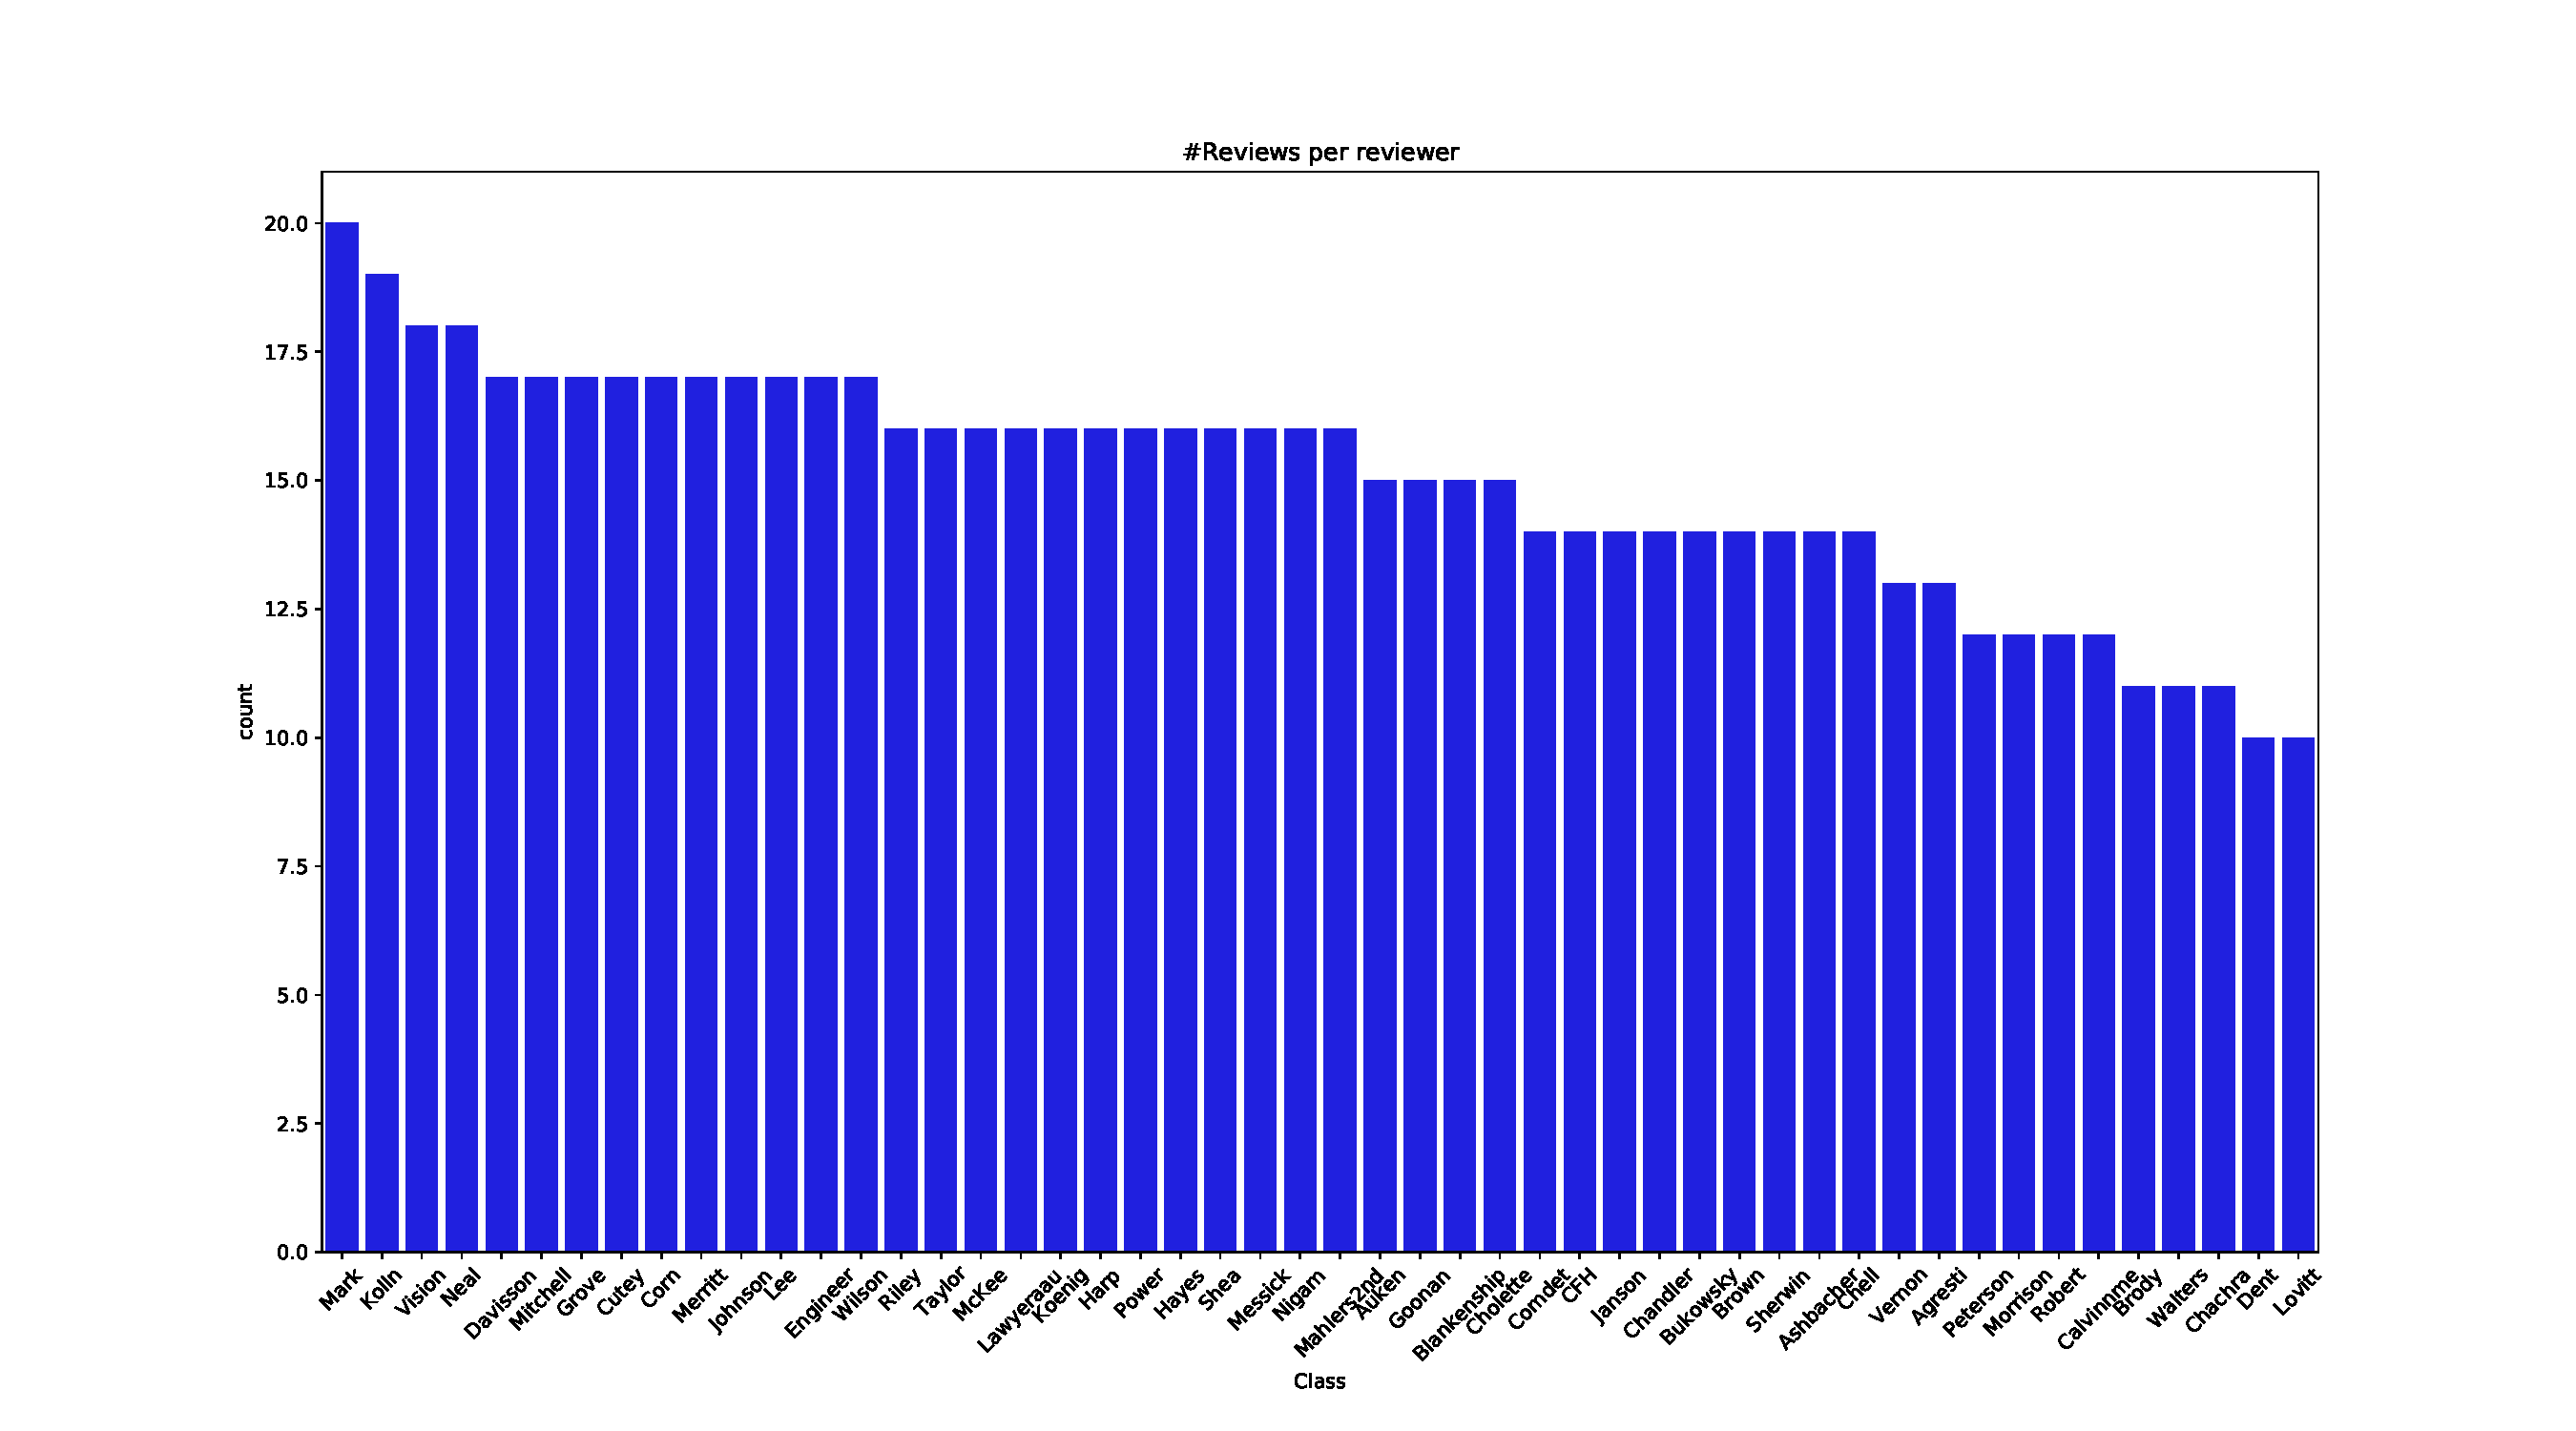
\includegraphics[width=1.0\linewidth]{amazon/Instances_per_class.pdf}
%\end{picture}
\end{minipage}
\caption{Instances per class}
\label{Fig::Instances_per_class}
%\end{minipage}
\end{figure}
%
\subsection{Pre-Processing}
There are no missing values in the dataset. The unique ID has been deleted from the data set as has no relevance to the class. The text vectors have values differentiating of a mean of 250 occurrences per instance to 1 occurrence in the entire dataset. With 250 occurrences per instance it appears as though stop words have not been deleted from the dataset, however as we do not have the raw data available we cannot be certain. 
\newline
We sort the vectors from highest number of total occurrences to the smallest number of total occurrences. Words which only occur in one instance can be seen as unique identifier to one author. By sorting the data we enable, to train our model leaving some of the first and last columns out and test whether this improve the model. The different scenarios taken into account can be seen in figure \ref{Fig::Descriptioon of scenarios}
\newline
In figure \ref{Fig::Distribution sum of vectors} one can see the distribution of the sum of the vectors. On average a word appears 309 times in all reviews, however there is a word which appears 187520 times, from 49 to 410 times in a review.
\newline
Two transformations to the dataset have been applied in order to flatten the weight of words which occur more often in one instance. The first transformation is the natural logarithm. The dataset will be transferred into $ln(X)+1$. The one is added to each entry to ensure 0 entries stay 0. The second transformation is a binary translation wher $x_{i,j}=1$ when $x_{i,j}>1$. The scenarios will be ran for both transformations as well.  
%
\begin{figure}
\begin{minipage}[t]{0.3\textwidth}
\begin{tabular}{lr}
\toprule
{} &	Sum of vectors \\
\midrule
count &   10000.000000 \\
mean  &     308.859700 \\
std   &    2419.468303 \\
min   &       0.000000 \\
25\%   &       9.000000 \\
50\%   &      21.000000 \\
75\%   &     220.000000 \\
max   &  187520.000000 \\
\bottomrule
\end{tabular}
\caption{Distribution sum of vectors}
\label{Fig::Distribution sum of vectors}
\end{minipage}
%
\begin{minipage}[t]{0.6\textwidth}
\begin{tabular}{lll}
\toprule
{} &   Scenario &  Scenario description \\
\midrule
0 &      10000 & Select all 10000 attributes   \\
1 &       8000 & select the first 8000 attributes  \\
2 &       6000 & select the first 6000 attributes   \\
3 &   50:10000 & select the 50th till the 10000th attribute   \\
4 &    50:8000 & select the 50th till the 8000th attribute    \\
5 &    50:6000 & select the 50th till the 6000th attribute    \\
6 &  100:10000 & select the 100th till the 10000th attribute    \\
7 &   100:8000 & select the 100th till the 8000th attribute    \\
8 &   100:6000 & select the 100th till the 6000th attribute	\\ 
\bottomrule
\end{tabular}
\caption{Description of different scenarios}
\label{Fig::Descriptioon of scenarios}
\end{minipage}
\end{figure}
%
\subsection{Parameter-Tuning}
First we will split the data in two parts. One part, 90 \%, for training and avlidation of the model with different parameters and the second part, 10\%, to test the models afterwards. To extract the test set, the hold out strategy has been used.
\newline
To split the rest of the data in a training dataset, and a validation dataset, both, the hold out strategy and the cross validation using 10-fold have been used. For the hold out a division of 80\% training and 20\% validation has been 
The results of the model on the validation sets are used to tune the parameters on the model.
\newline
In order to set the scenarios and the parameters used we will make use of the average F1-score. 
%
\newline
\textbf{Perceptron}:We determine the base parameters for the perceptron, alpha as 0.0005, eta as 1 penalty='none' and the max iterations are equal to 100. The results of the 9 scenarios for all tranformations can be found in figures  \ref{Fig::Perceptron parametertuning} using both the hold out and cross validation strategy.
All train sets of the transformed datasets havean F1-score of 100. For the non-transformed dataset a score of 100 was only obtained when high occurring words were deleted.. 
\newline
Comparing the F-1 of the test set of the different transformations binary transformation performs the worse in all scenarios. The logarithmic transformations performs better when we do not delete the words with high occurrences. After removing the top 50 words the F1-score of the $X$ dataset is higher than the$ln(X)+1$ dataset. This can be explained due to the fact that transforming the data into logarithmic values has the highest effect on the words which occur most often.
\newline
A clear difference can be seen between the performance of the hold out and the cross validation runs. The cross validation run has more stable result, where the hold out fluctuates more. Due to the high amount of classes, 50, and the relative low amount of instances it can happen that classes are not represented in the test set, some classes only appear 10 times in the entire dataset. The performance is sensitive to the chosen validation and train set. With using the cross validation the entire dataset is used (except the part left out for testing) and the influence of chance decreases. In order to tune the hyper parameters we will use the cross validation and look at the results of the validation set. Due to the high complexity of the data, and a relative little instances the classifiers can train the model to fit training data exactly, even with linear classifiers. Therefore the results on the training data cannot be compared. 
\newline
For the parameter tuning of on the perceptron classifier scenario 3 of the non-transformed dataset is chosen as it has the best f1-score.
%
\begin{figure}[t]
\begin{minipage}[t]{0.33\textwidth}
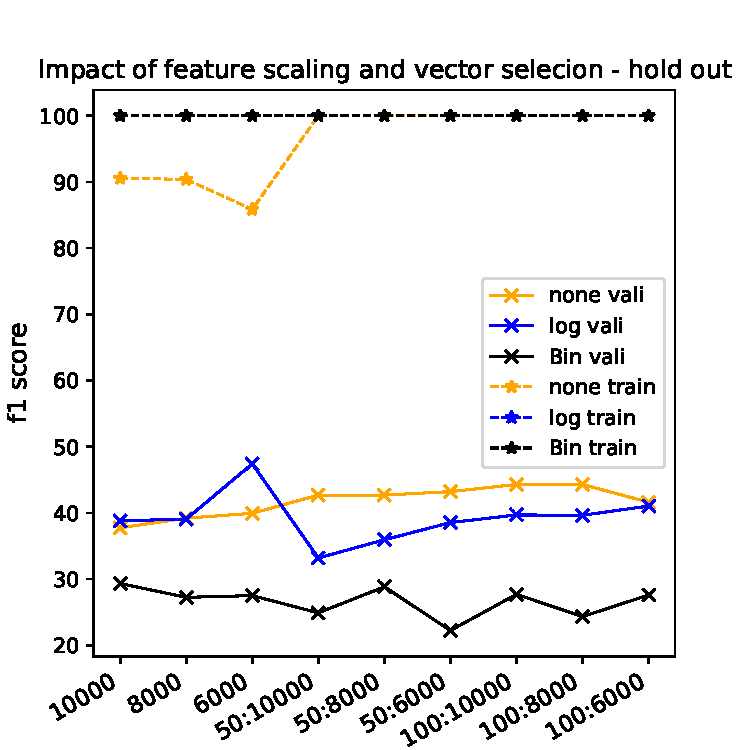
\includegraphics[width=1\linewidth]{amazon/perc_scaling_vect_selection_HO.pdf}
\end{minipage}
\begin{minipage}[t]{0.33\textwidth}
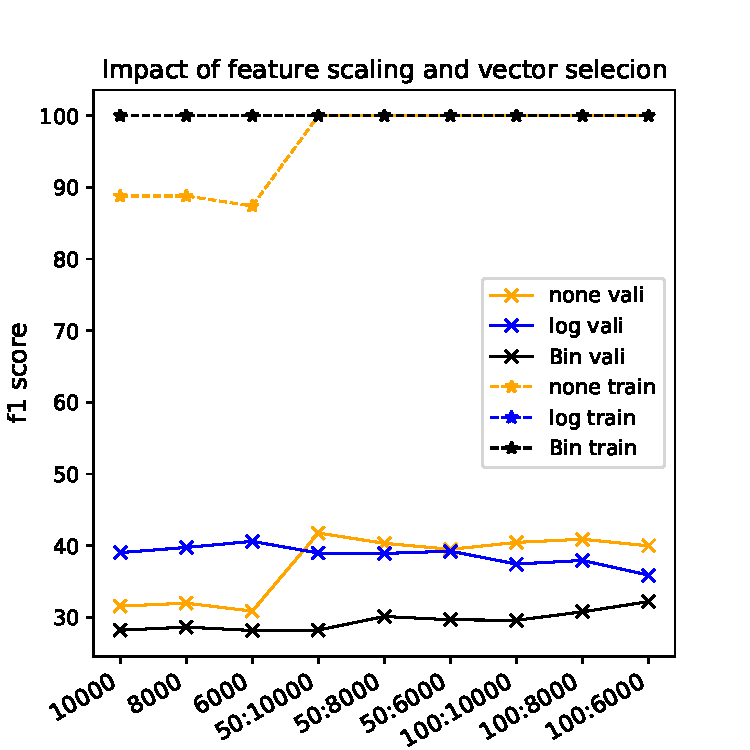
\includegraphics[width=1\linewidth]{amazon/perc_scaling_vect_selection.pdf}
\end{minipage}
\begin{minipage}[t]{0.33\textwidth}
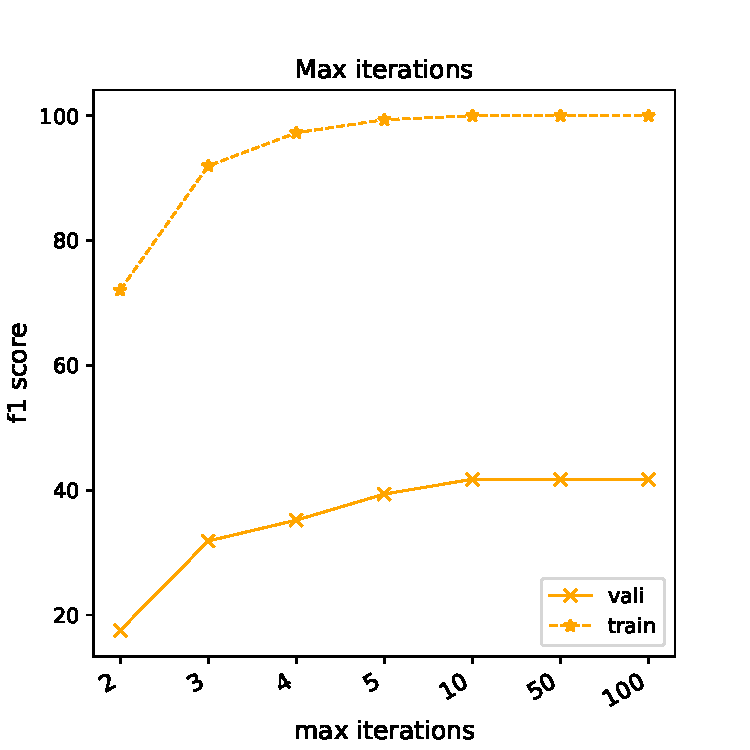
\includegraphics[width=1\linewidth]{amazon/Per_max_iterations_2.pdf}
\end{minipage}
\begin{minipage}[t]{0.33\textwidth}
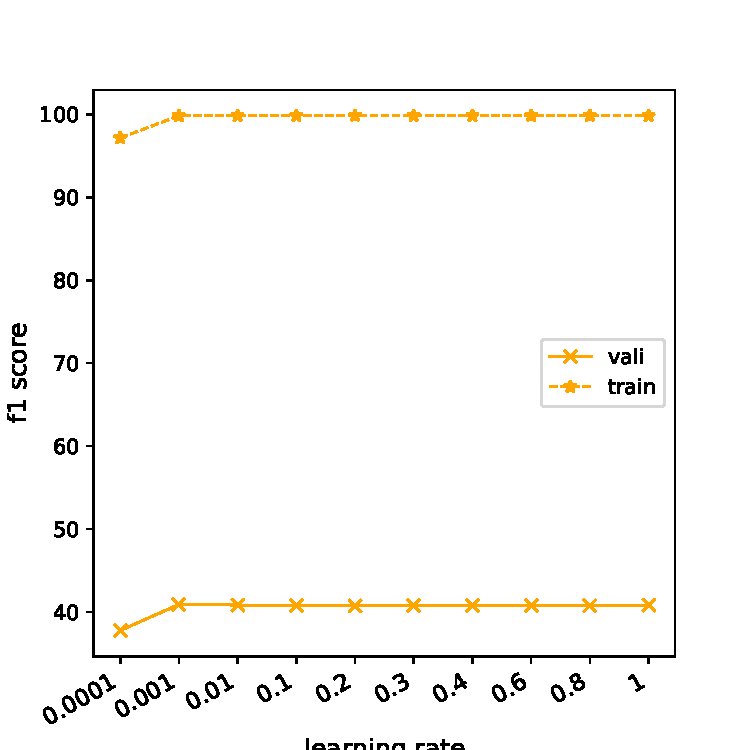
\includegraphics[width=1\linewidth]{amazon/Per_learning_rate2.pdf}
\end{minipage}
\begin{minipage}[t]{0.33\textwidth}
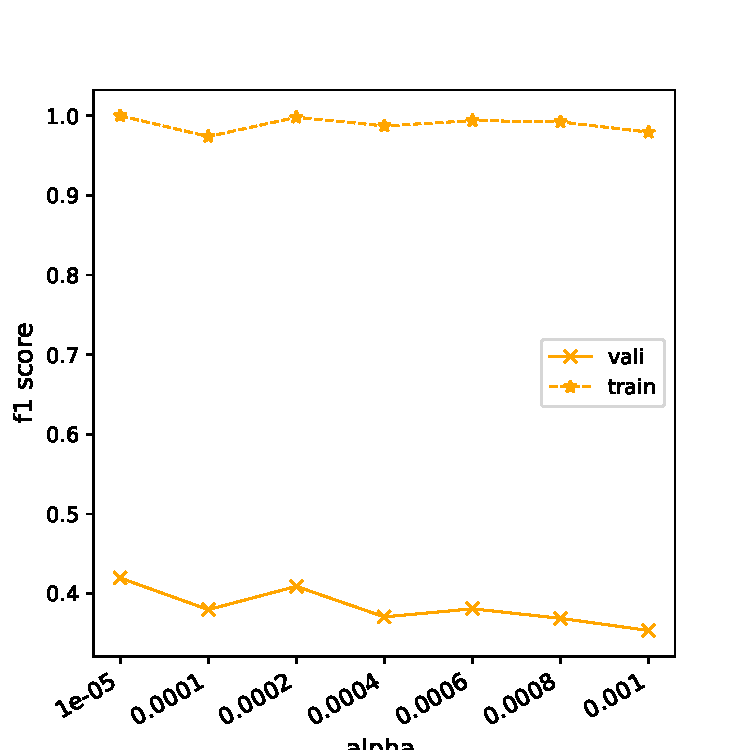
\includegraphics[width=1\linewidth]{amazon/Per_alpha2.pdf}
\end{minipage}
\caption{Parameter tuning perceprton}
\label{Fig::Perceptron parametertuning}
\end{figure}
%
The first parameter we tune is the maximum number of iteration maxiter. We test for values  maxiter $\in \{2, 3, 4, 5, 10, 50, 100\}$. It can be seen that after 10 iterations the training set has a perfect fit, and the validation set has the highest performance. Therefore, we take $maxiter=10$ for the next parameter tuning.
\newline
Next the model is trained for different learning rates ($eta0$), where $ eta0 \in \{1^{-4}, 1^{-3}, 0.01, 0.1, 0.2, 0.3, 0.4, 0.6, 0.8, 1\} $. The model is only influences slightly by the different learning rates.The highest performance was obtained wit a learning rate of 0.01. 
\newline
Finally a regularization term has been introduced.We ram $\alpha$ was set to be $ \in \{ 1e^{-4}, 1e^{-3}, 0.01, 0.5, 1\}$. The f1-score for both the training set as well as the validation set dropped rapidly after $1^{-3}$. Therefore, a second run with $\alpha \in  \{1e^{-5}, 1e^{-4}, 0.0002, 0.0004, 0.0006, 0.0008, 1e{-3}\}$ has been done. For $\alpha=0.00001$, the validation performs best with an f1 score of  $42.0\%$. 
%
We run our final model for the test set with the best parameters settings from the parameter tuning. The parameters are as follows maximum number of iterations is 10, $eta0=0.0011$, the regularization term is l1, with an $\alpha$ of $0.00001$ against the test set. This results in an accuracy of $53.3\%$ and a f-1 score of $49.8\%$. 
%
\begin{figure}[t]
\begin{minipage}[t]{0.33\textwidth}
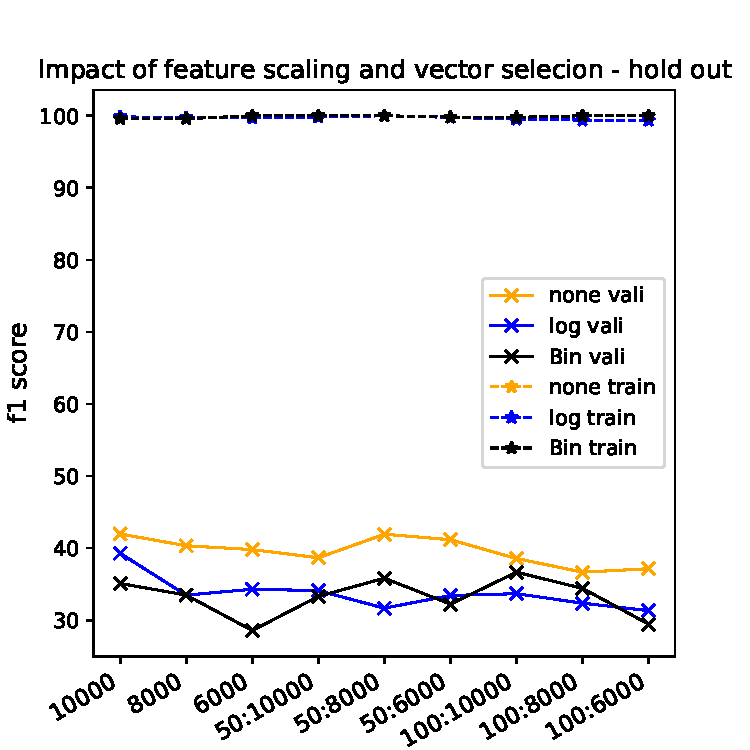
\includegraphics[width=1\linewidth]{amazon/RF_scaling_vect_selection_HO.pdf}
\end{minipage}
\begin{minipage}[t]{0.33\textwidth}
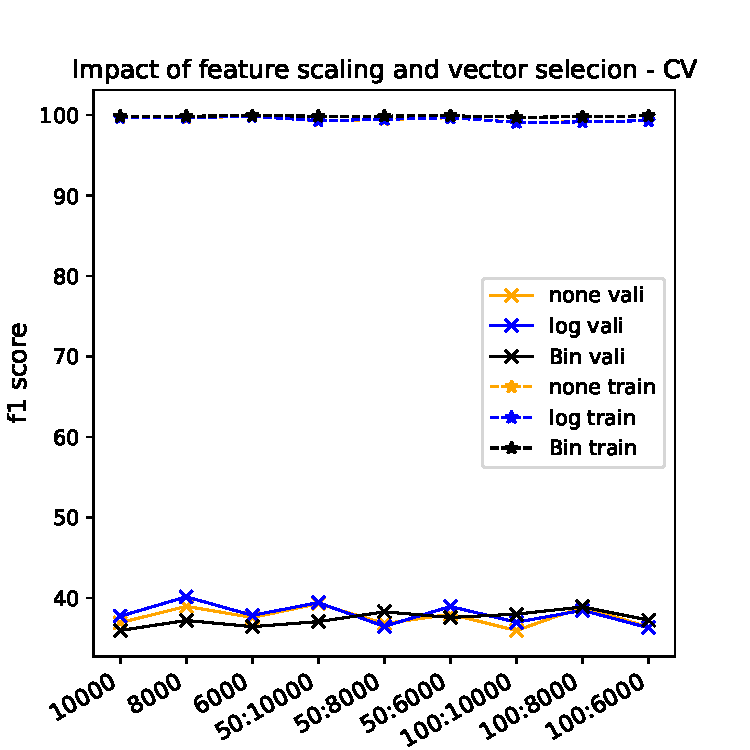
\includegraphics[width=1\linewidth]{amazon/RF_scaling_vect_selection_CV.pdf}
\end{minipage}
\begin{minipage}[t]{0.33\textwidth}
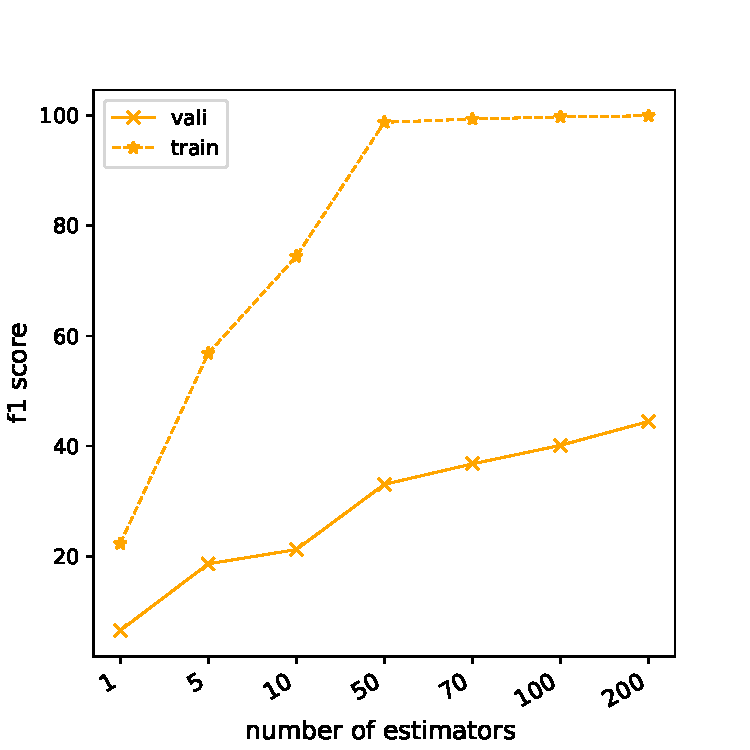
\includegraphics[width=1\linewidth]{amazon/RF_nestimators.pdf}
\end{minipage}
\begin{minipage}[t]{0.33\textwidth}
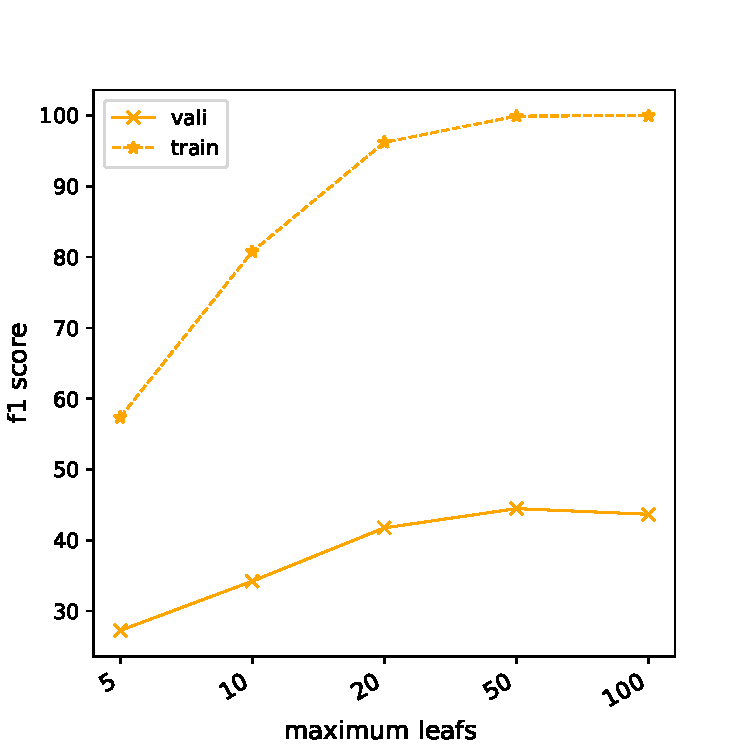
\includegraphics[width=1\linewidth]{amazon/RF_max_leafs.pdf}
\end{minipage}
\begin{minipage}[t]{0.33\textwidth}
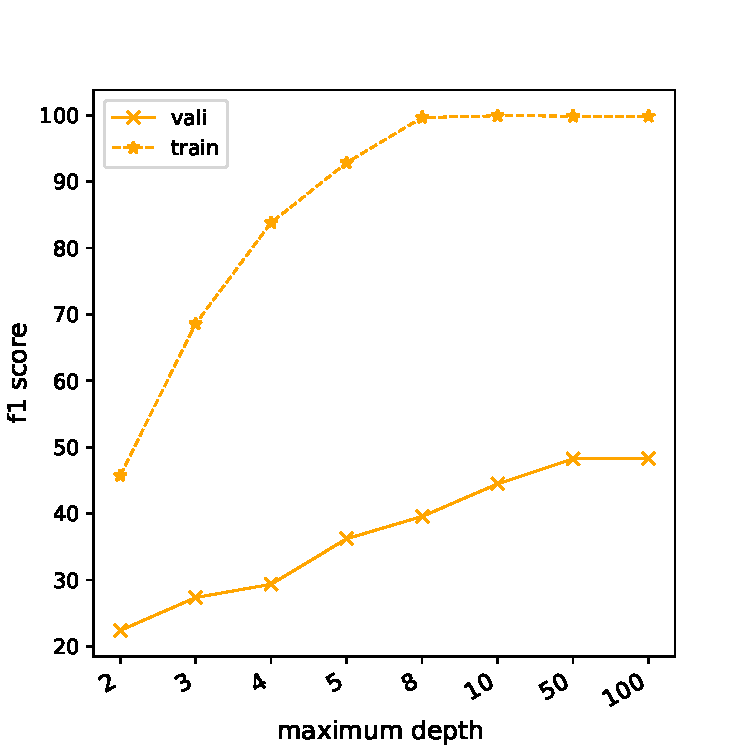
\includegraphics[width=1\linewidth]{amazon/RF_max_depth.pdf}
\end{minipage}
\begin{minipage}[t]{0.33\textwidth}
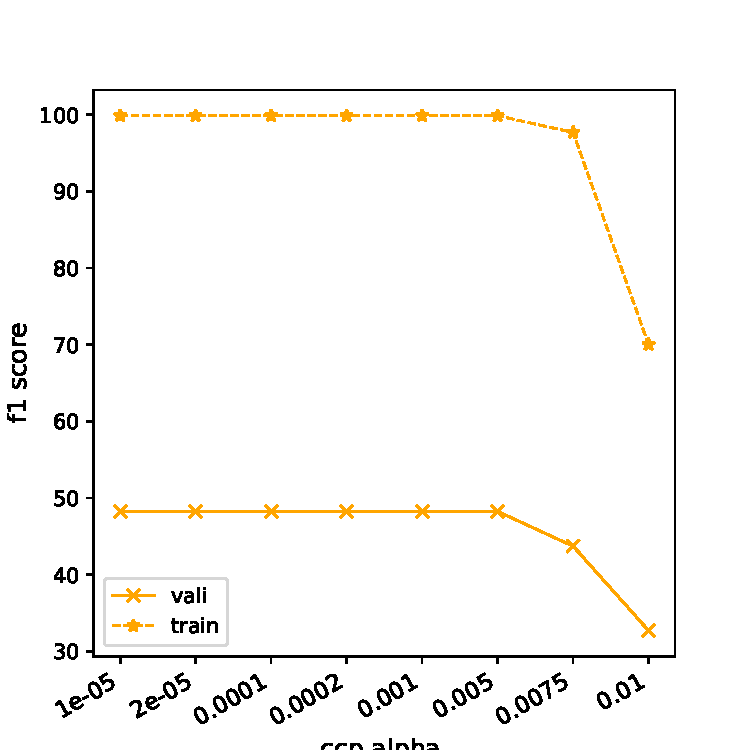
\includegraphics[width=1\linewidth]{amazon/RF_ccp_alpha.pdf}
\end{minipage}
\caption{Parameter tuning random forest}
\label{Fig::Random forest parameter tuning}
\end{figure}
%
\newline
\textbf{Random forest}: The second classifier is the random forest classifier. The base parameter settings are the following:$ccp \alpha = 0$, $max leaf = 50$, $max depth = 10$ and
$number of estimators = 100$. The results of the different scenarios for hold out and cross validation can be found in the figures \ref{Fig::Random forest parameter tuning}. The best accuracy is obtained scenario 2 on the natural logarithmic dataset with an f1-score of $40.15\%$ in the cross validation. For the first scenarios the logarithmic transformation performs best. Starting at scenario 4 the performances come closer together and there is no transformation which out performs the other. 
\newline
The following hyper parameters have been tested: number of estimators, the maximum depth, maximum leafs and the complexity cost parameter, ccp alpha. Starting with the number of estimators, the number of trees, given n estimators $\in \{1,5,10, 50, 70, 100, 200\}$. 
\newline
Both the train set and the validation set achieve an higher performance, for all scoring methods, whenever the number of estimators increases. The number of estimators is set to 200.
\newline
The second hyper parameter is the maximum number of leafs per branch, we test $max leafs \in \{5,10, 20, 50, 100\}$ The accuracy increases when the number of leafs increase to 50, with 100 all performances increase for the training set, but not for the test set. The model is over fitting. The maximum number of leafs is set to 50.   
\newline
After the number of trees and the leafs per branch, the depth of each tree is determined. where $max depth \in \{2, 3, 4, 5, 8, 10, 50, 100\}$. The f1-score for the training set is highest with a maximum depth of $10$. The f1-score for the validation set is highest with a maximum depth of $50$ or a $100$, the same scores are obtained. The maximum depth is set to $50$. 
\newline
Last, we tune the minimal cost complexity pruning parameter. We test for $ccp  \alpha \in \{1e-5, 2e-5, 1e-4, 2e-4, 1e-3, 5e-3, 75e-4, 1e-2\}$. It can be seen that for $ccp \alpha < 0.005$ the pruning does not cost. However, for $ccp \alpha > 0.005$ both the train and the test have reduced scores. Therefor, we will set $ccp \alpha=0.005$.   
%
The final model is now tested on the validation data with the following parameter settings:
$n estimators = 200$ ,$max_leaf = 50$, $max_depth = 50$ and $ccp \alpha = 0.005$. This results in an f1-score of $51.8\%$.
\newline 
\textbf{Naive Bayes}: The third classifier is the multinominal Naive Bayes classifier. For the base run we set $\alpha$ equal to 1. The nine scenarios are run for both hold out and cross validation. A clear pattern can be seen in the result. The accuracy of the non transformed dataset clearly out performs the logarithmic and the binary transformations. Furthermore it can be seen that including less vectors improves the model, both the first and the last vectors from the dataset. As the best results are obtained in scenario 8, additional scenarios are ran excluding additional vectors from the beginning and the end.  
\newline
First 5 additional scenarios are created excluding more vectors in the end. The best results are obtained with scenario 11, and 12. Another 10 scenarios are considered leaving the first 150, 200, 250, 300 and 350 vectors out until the 4000th and the 4500th vector. The accuracy can be found in table \ref{Fig::Naive Bayes parameter tuning}. the best accuracy is obtained in scenario 250 closely followed by scenario 22.
\newline
The first 9 scenarios have been ran for different smoothing priors. We ran the model for alpha's $\in \{1e{-3}, 1e{-2}, 1e{-1}, 0.5, 1, 10, 100, 1000\}$. All results are equal for all alphas.  
\begin{figure}[h]
\begin{minipage}[t]{0.33\textwidth}
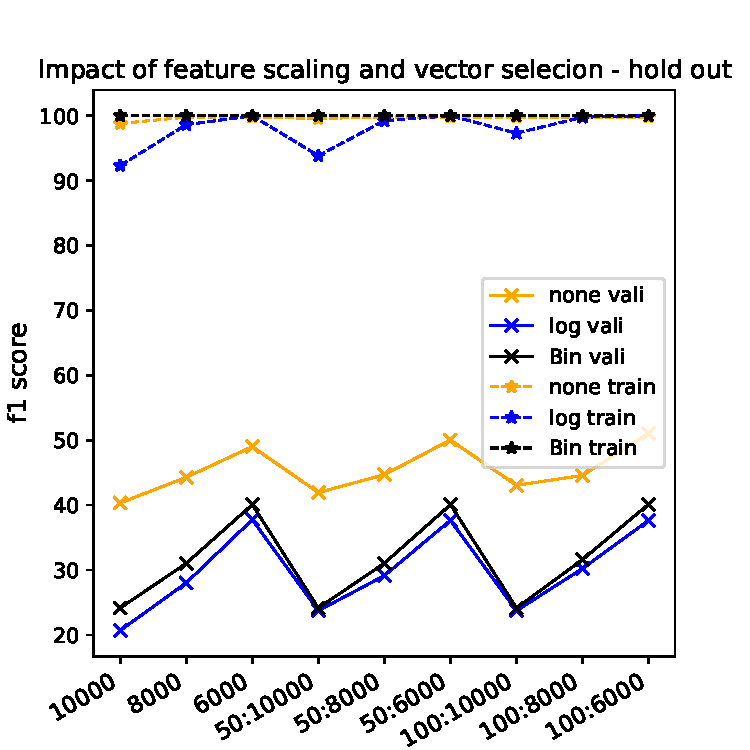
\includegraphics[width=1\linewidth]{amazon/NB_scaling_vect_selection_HO.pdf}
\end{minipage}
\begin{minipage}[t]{0.33\textwidth}
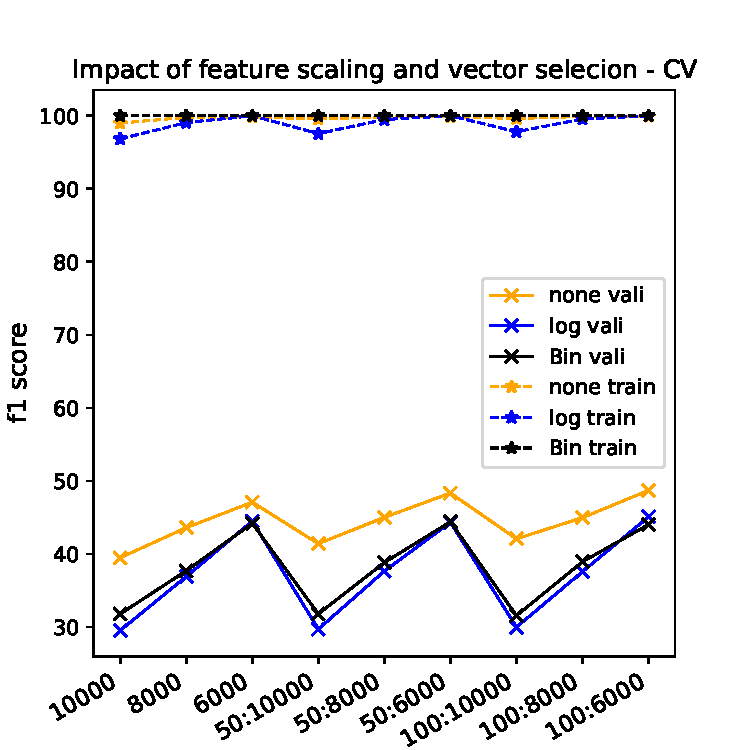
\includegraphics[width=1\linewidth]{amazon/NB_scaling_vect_selection_CV.pdf}
\end{minipage}
\begin{minipage}[t]{0.33\textwidth}
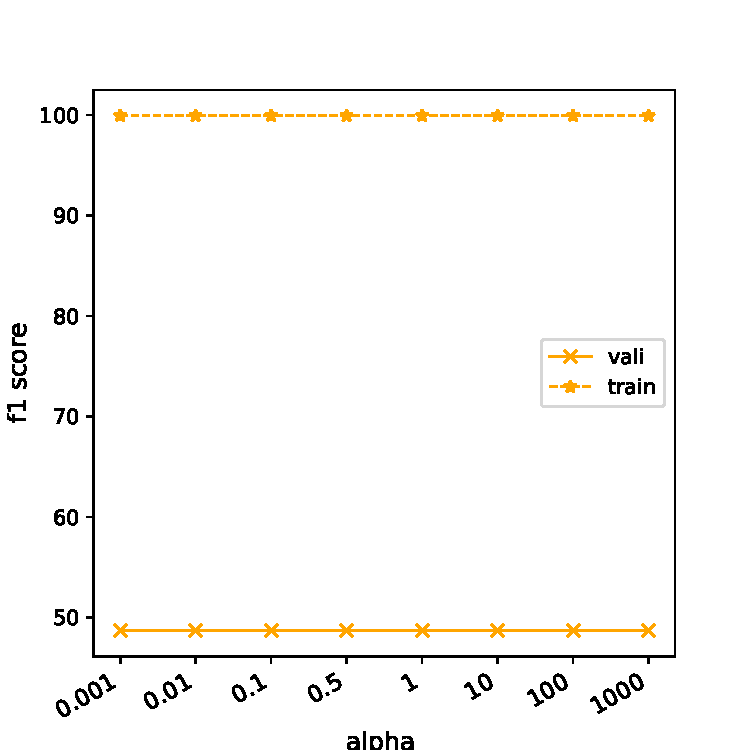
\includegraphics[width=1\linewidth]{amazon/NB_alpha.pdf}
\end{minipage}
\begin{minipage}[t]{0.33\textwidth}
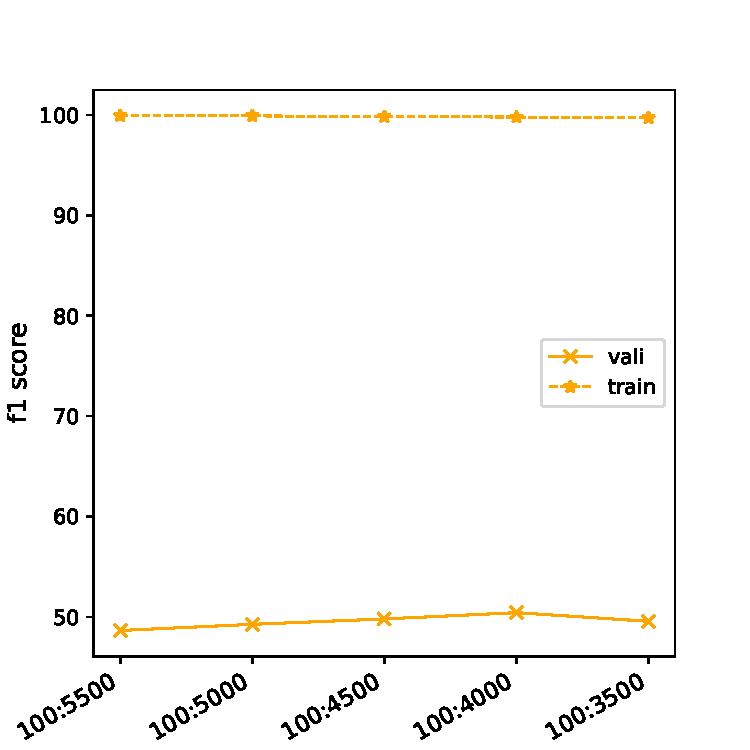
\includegraphics[width=1\linewidth]{amazon/NB_Xrange2.pdf}
\end{minipage}
\begin{minipage}[t]{0.33\textwidth}
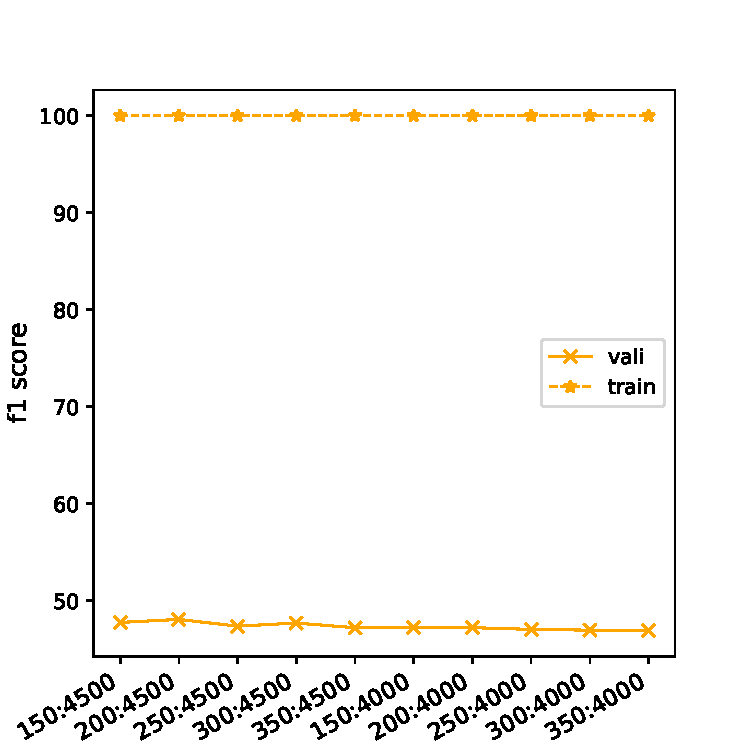
\includegraphics[width=1\linewidth]{amazon/NB_Xrange3.pdf}
\end{minipage}
\begin{minipage}[t]{0.33\textwidth}
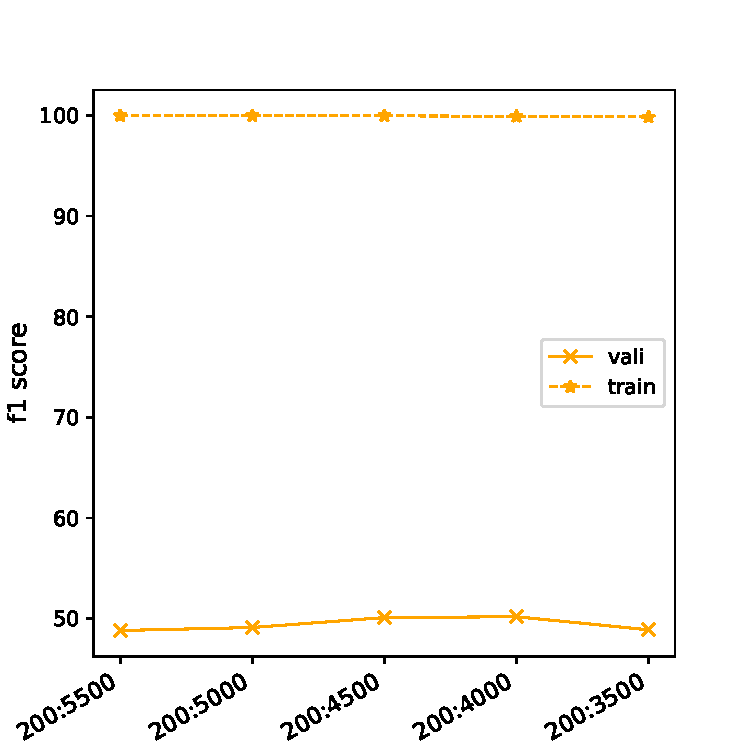
\includegraphics[width=1\linewidth]{amazon/NB_Xrange4.pdf}
\end{minipage}
\caption{Parameter tuning Naive Bayes.}
\label{Fig::Naive Bayes parameter tuning}
\end{figure}

\section{Congressional Voting Dataset}
\subsection{Dataset Description}
\subsection{Pre-Processing}
\subsection{Parameter-Tuning}
\subsection{Performance-Analysis}


\section{Email Spam Dataset(\href{https://www.kaggle.com/nitishabharathi/email-spam-dataset}{link to dataset})}


\subsection{Dataset Description}
The task of the email spam dataset is to predict if an email is spam or not. The link above contains three datasets from which we choose two, namely the \texttt{lingSpam.csv} and \texttt{enormSpamSubset.csv} for our project, since they have no missing values and the same layout. The dataset contains 12604 emails where 43.11% are spam and 56.89% are non-spam emails.The basic structure of emails can be seen in figure \ref{tab_spam0}.

\begin{figure}[h]
  \begin{tabular}{ | c | p{15cm} | c |}
    \hline
    Index & Body & Label \\
    \hline
    100 & 
    Subject: inexpensive online medication here
 pummel wah springtail cutler bodyguard
 we ship quality medications overnight to your door !...
    & 1 \\ \hline
    6006
    &
    Subject: organizational changes
 we are pleased to announce the following organizational changes :
 enron global assets and services
 in order to increase senior management focus on our international businesses... 
    & 0 \\
    \hline
    \end{tabular}
    \caption{Structure of the Email-Spam Dataset}
    \label{tab_spam0}
  \end{figure}
Every email has a binary target-label assigned, such that a 0 marks non-spam and a 1 marks spam emails. In figure \ref{spamfig_fig0} the distribution of the characters per email is shown. We see that most emails have a lenght in the range of 100 to 10.000 characters.

\begin{figure}
\begin{minipage}[t]{0.3\textwidth}
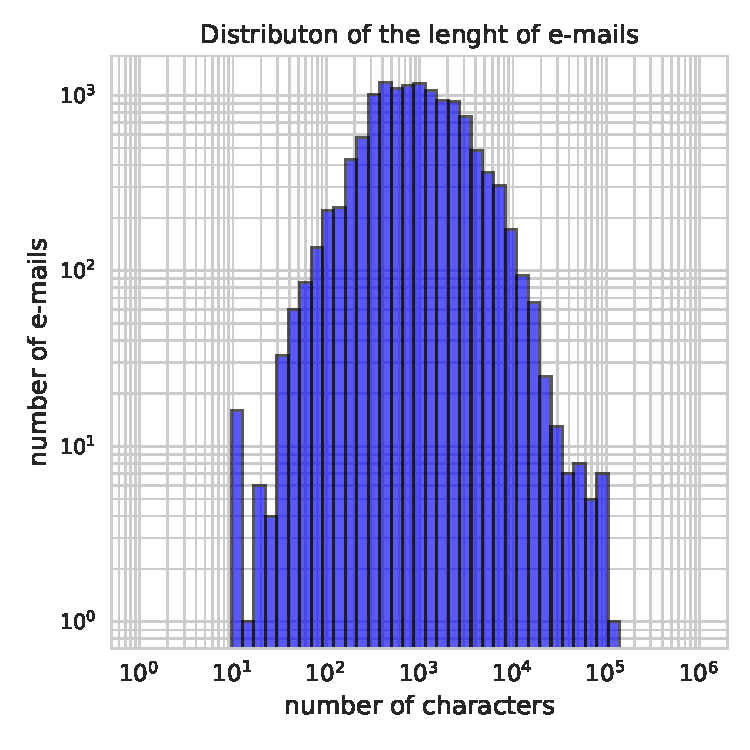
\includegraphics[width=1\linewidth]{email_spam/char_count.pdf}
\end{minipage}
\begin{minipage}[t]{0.3\textwidth}
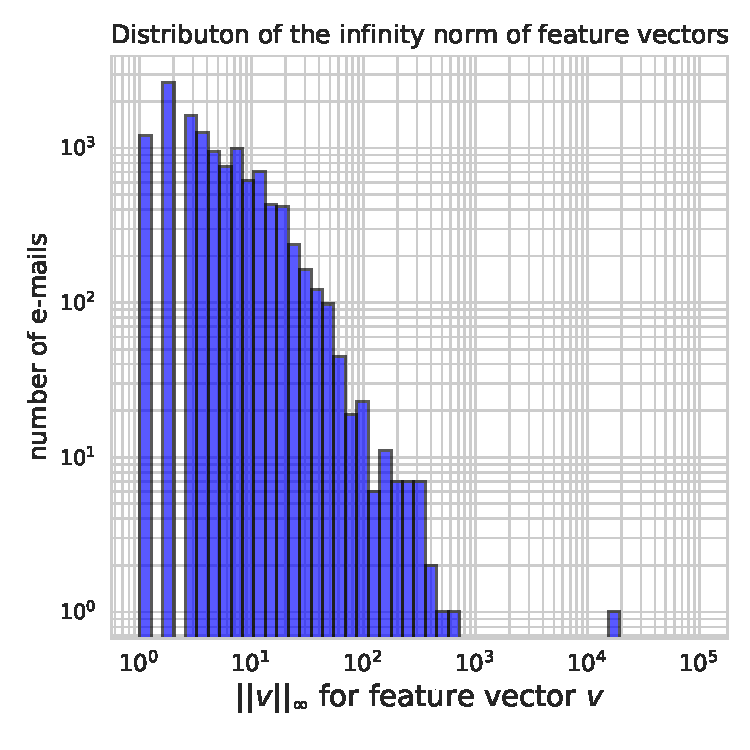
\includegraphics[width=1\linewidth]{email_spam/word_count.pdf}
\end{minipage}
\begin{minipage}[t]{0.3\textwidth}
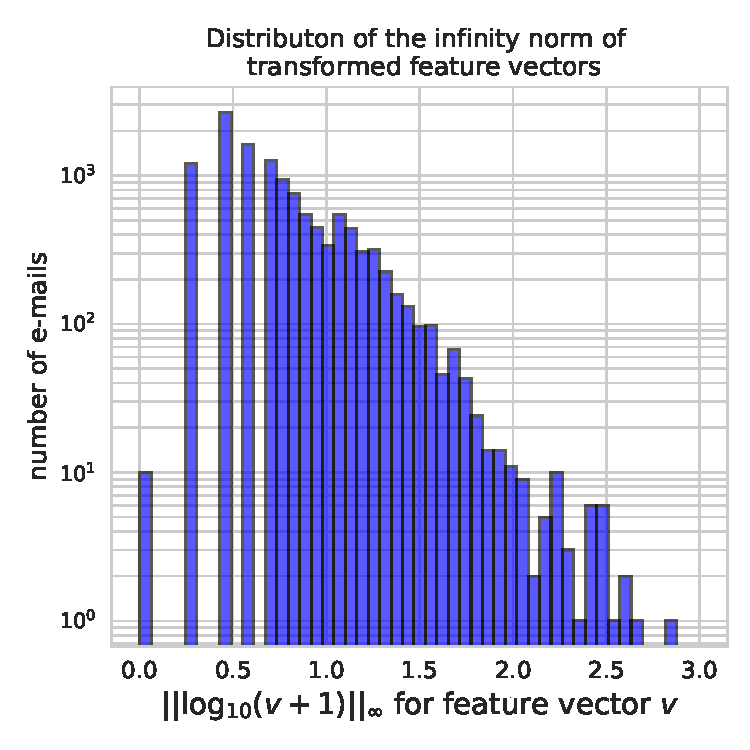
\includegraphics[width=1\linewidth]{email_spam/word_transformed_count.pdf}
\end{minipage}
   \caption{left: Distribution of e-mail lenghts, middle: Distribution of maximum norm in extracted word vectors with lenght 8000, right: Distribution of maximum norm in extracted word vectors with lenght 8000 after removing outlyers and applying logarithmic transformation}
\label{spamfig_fig0}
\end{figure}

\subsection{Pre-Processing}
In the dataset are 213 duplicate emails that we first remove and then peform the train/test-split where the trainset size is $20\%$ of the original dataset. Next we apply the Bag of Words feature extractor to each email. The algorithm converts every email to a vector $v\in\mathbb{Z}^N$ of intergers. First we create a list of all words and count their occurences in all emails. Then we take the $N$ most common words and count the occurences of the most common words in every email to get $v$. Before applying the Bag of word extractor we pre-process emails by the following steps:1. remove links (http...), 2. remove all characters exept alphabetical chars and numbers, 3. convert uppercase to lowercase, 4. split text-bodys into separate words, 5. lemmatize all words, 6. remove stopwords. For the steps 5., 6. we use nltk python package. By the preprocessing we reduce the number of distinct words from 126019 to 103759 words. 

In figure \ref{spamfig_fig0} middle we see the distribution of the maximum norm of the extracted vectors. One can identify that the maximum norm spans several orders of magnitude from $0$ to $10^5$. Especially there is only one vector $v$ with $||v||_\infty>10^4$. Outlyers with $||v||_\infty>10^3$ are therefor removed in the testset. Additionally we apply the logarithmic transformation $\log_{10}(x+1)$ to all the elements of a vector and obtain a $||\cdot||_\infty$ distrubution that is bounded by the maximum magnithude. Note that we add $1$ to all components of a vector since this component is $0$ after the logarithmic transformation. The distribution after the transformation is shown in figure \ref{spamfig_fig0} right.




\subsection{Parameter-Tuning}
For the parameter Tuning we further split the trainingset into a $20\%$ validation and $80\%$ trainingset. The model fitting is done on the trainingset and the parametertuning with regard to the performance on the validation set. We select parametervalues by the cross validation performance, since we assume this performance if more stable when compared to the holdout validation, that might be to optimistic ore pessimistic. Since the task is to distinguish spam and non-spam emails and we assume that misslabeling important non-spam emails is just as importnant as not misslabeling potentially harmfull spam emails we make use of the F1-score as performance metric. This further makes sense since our dataset is relatively balanced as stated above.
%
\newline
\textbf{Perceptron}: We compare cross-validation with 10 splits to a holdout-validation. In figure \ref{spamfig_fig1} top left we see the influence of the scaling method on the f1-score of the perceptron algorithm. The binary scaling means that the transformed vectors have value 1 in a component if the original vectors component is nonzero and 0 otherwhise. Binary and logarithmic sclaing have the best performance in the cross validation, where the logarithmic scaling has slightly better performance on the trasining set. Therefore we choose the logarithmic scaling for the dataset. In figure \ref{spamfig_fig1} top middle the influence of the extracted features on the perceptron algorithm with default parameters is shown. The performance for the perceptron is optimal for 2000 features since the f1-score saturates for this feature number. Therefore we adapt this number of features and investigate the learing rate in figure \ref{spamfig_fig1} top right. Here the optimal learing rate is $0.1$ if we consider the cross-validation performance on the validaton set. Note that the holdout performance is not optimal for this value. The influence of the tolarance can be seen in \ref{spamfig_fig1} bottom left. For values lower than $0.001$ it has a constant f1-score that dropt for the cross validation on the validation set when we increase it. We can therefore fix the tolarance at $0.001$ and investigate the maximum number of terations in \ref{spamfig_fig1} bottom middle. Surprisingly a low number of iterations causes the f1-score to increase. We fix the maximum iteration for this purpose to 10.

\begin{figure}
\begin{minipage}[l]{0.3\textwidth}
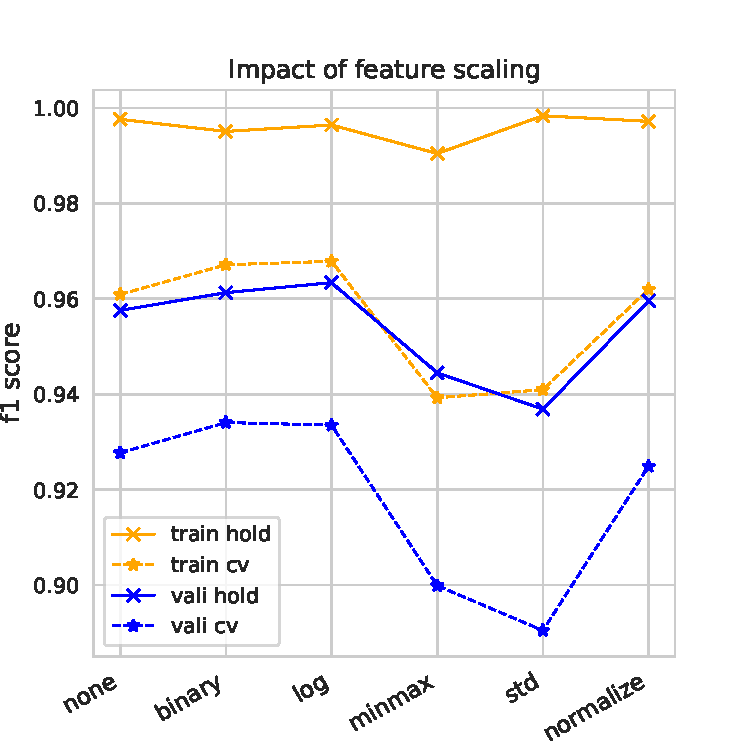
\includegraphics[width=1\linewidth]{email_spam/perc_scaling.pdf}
\end{minipage}
\begin{minipage}[l]{0.3\textwidth}
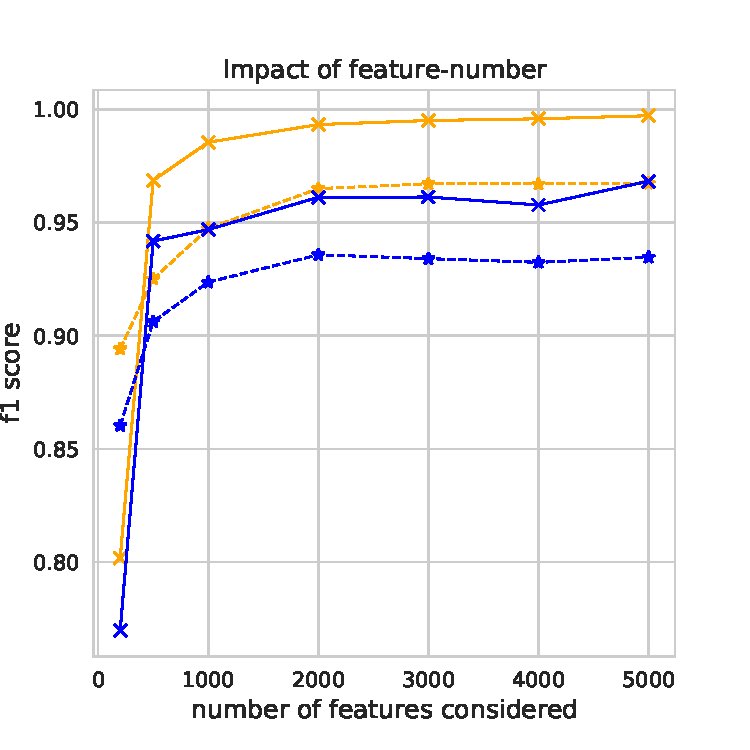
\includegraphics[width=1\linewidth]{email_spam/perc_features.pdf}
\end{minipage}
\begin{minipage}[l]{0.3\textwidth}
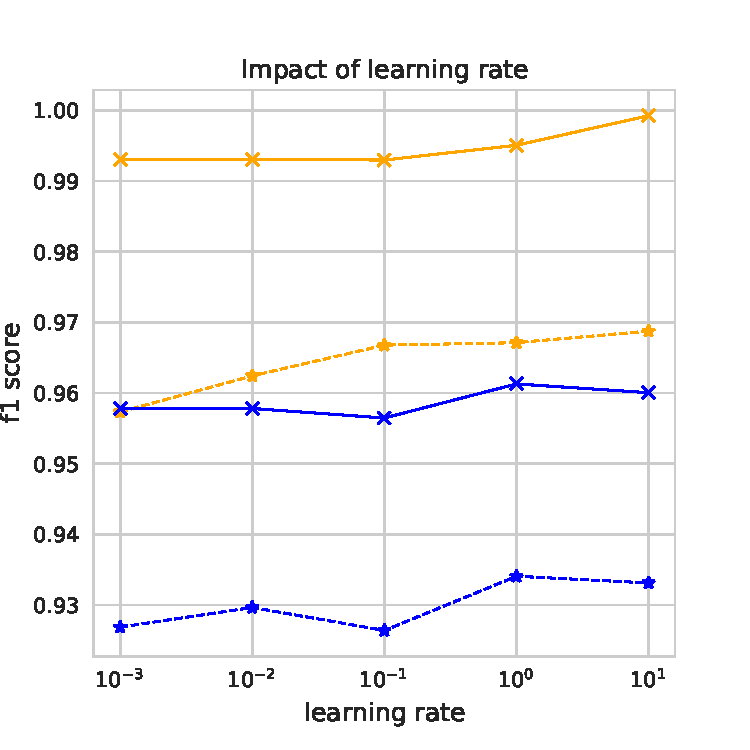
\includegraphics[width=1\linewidth]{email_spam/perc_learning_rate.pdf}
\end{minipage}\\
\begin{minipage}[t]{0.3\textwidth}
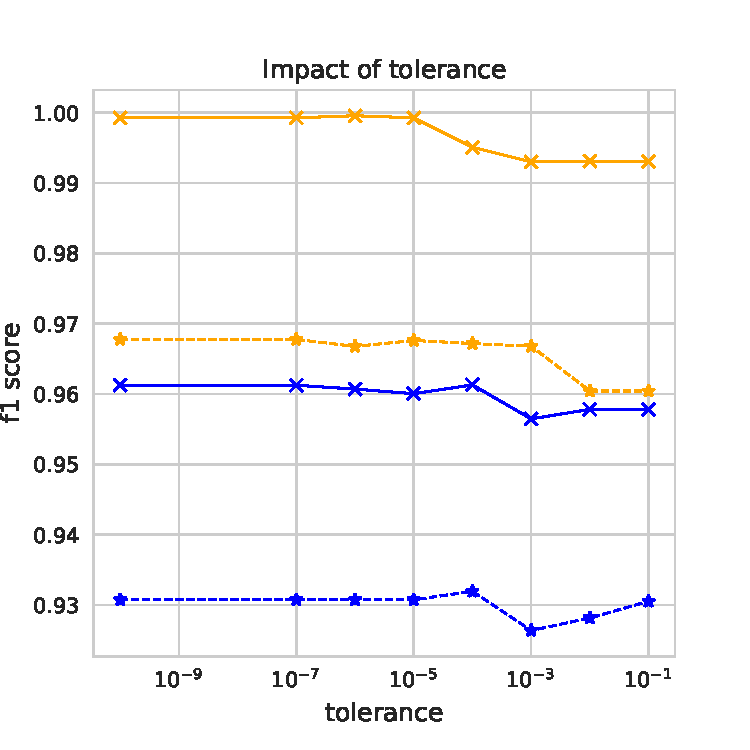
\includegraphics[width=1\linewidth]{email_spam/perc_tolerance.pdf}
\end{minipage}
\begin{minipage}[t]{0.3\textwidth}
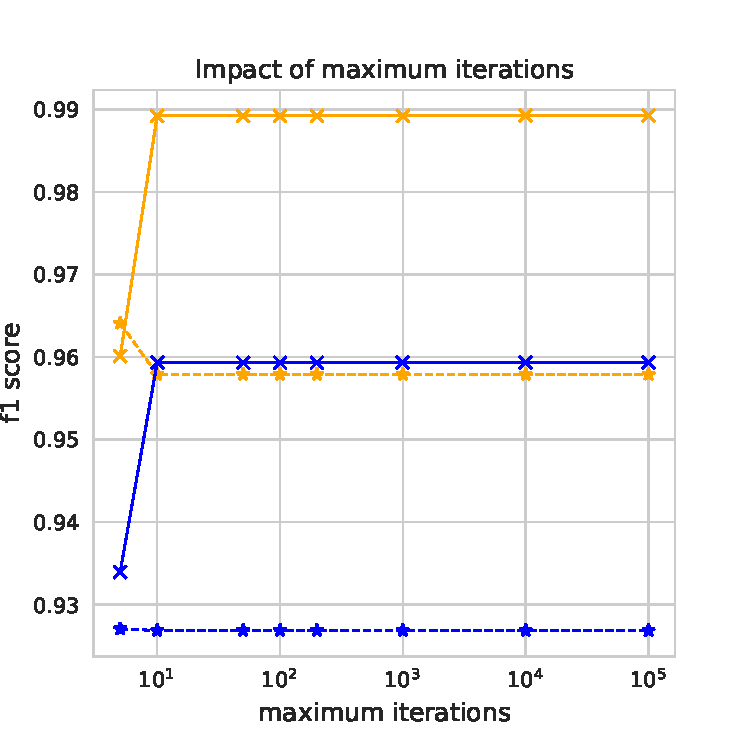
\includegraphics[width=1\linewidth]{email_spam/perc_maxiter.pdf}
\end{minipage}
\begin{minipage}[t]{0.3\textwidth}

\end{minipage}
   \caption{F1-score of Perceptron for different pre-processing parameters and model-parameters}
\label{spamfig_fig1}
\end{figure}

For the perceptron the cross validation yields always a more pessimistic performance when compared to the holdout-validation. As optimal parameters we have chosen: scaling method: logarithmic, extracted features: $2000$, learning rate: $0.001$, tolerance: $1e-6$. The f1-score on the testset is for this parameters: 0.97 for the holdout validation and 0.95 for the cross validation.
\newline
\textbf{Random forrest}:
Since the random forrest has much larger runtime compared to the other algorithms in this project we will not evaluate its performance on the training set and further set the number of validation steps in the cross validation to 4.

\begin{figure}
\begin{minipage}[l]{0.3\textwidth}
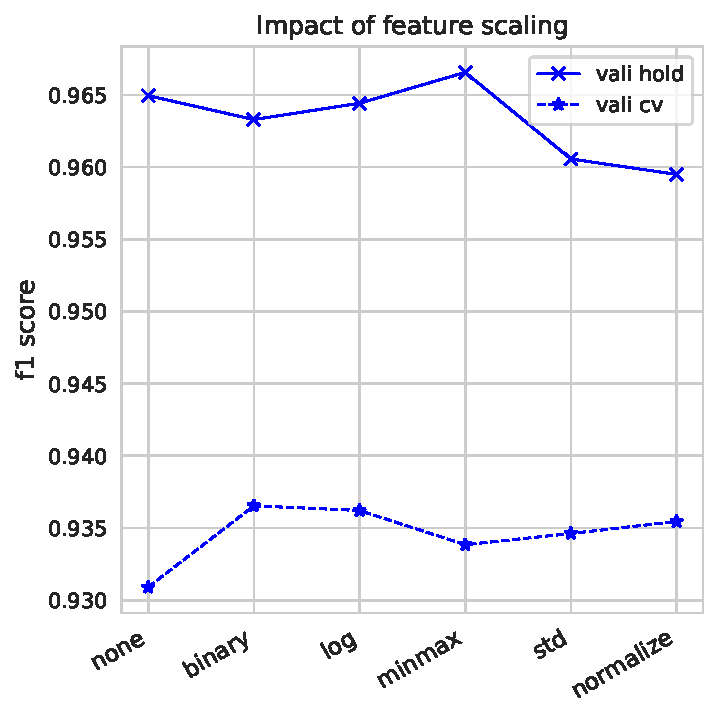
\includegraphics[width=1\linewidth]{email_spam/rnd_scaling.pdf}
\end{minipage}
\begin{minipage}[l]{0.3\textwidth}
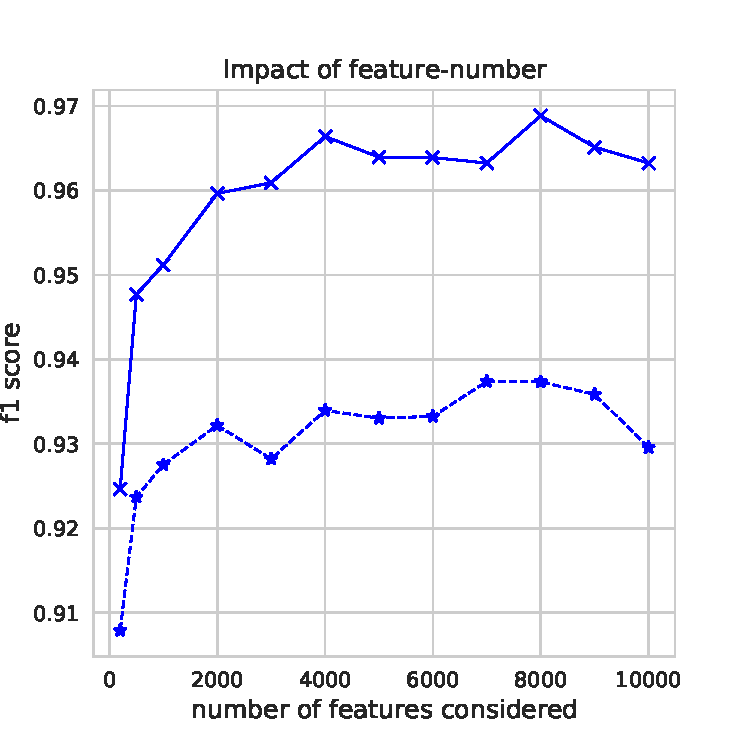
\includegraphics[width=1\linewidth]{email_spam/rnd_features.pdf}
\end{minipage}
\begin{minipage}[l]{0.3\textwidth}
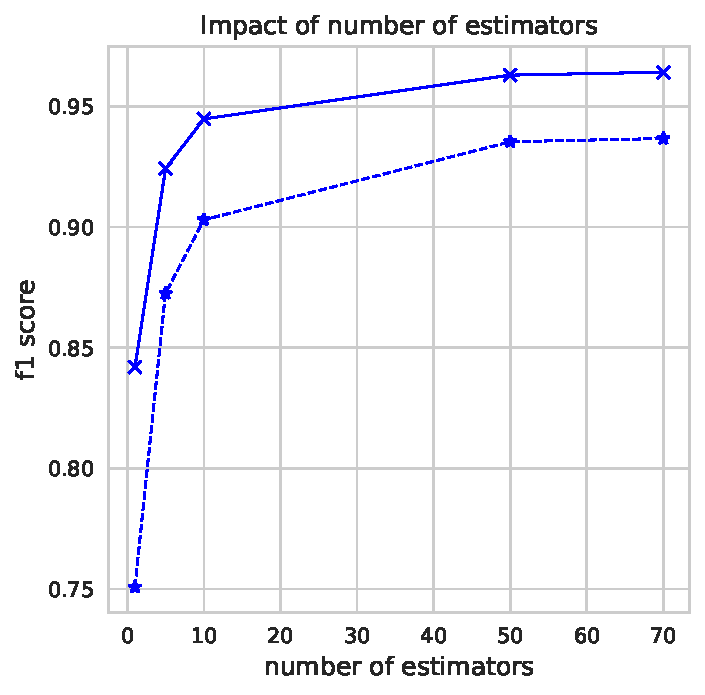
\includegraphics[width=1\linewidth]{email_spam/rnd_trees.pdf}
\end{minipage}\\
\begin{minipage}[l]{0.3\textwidth}
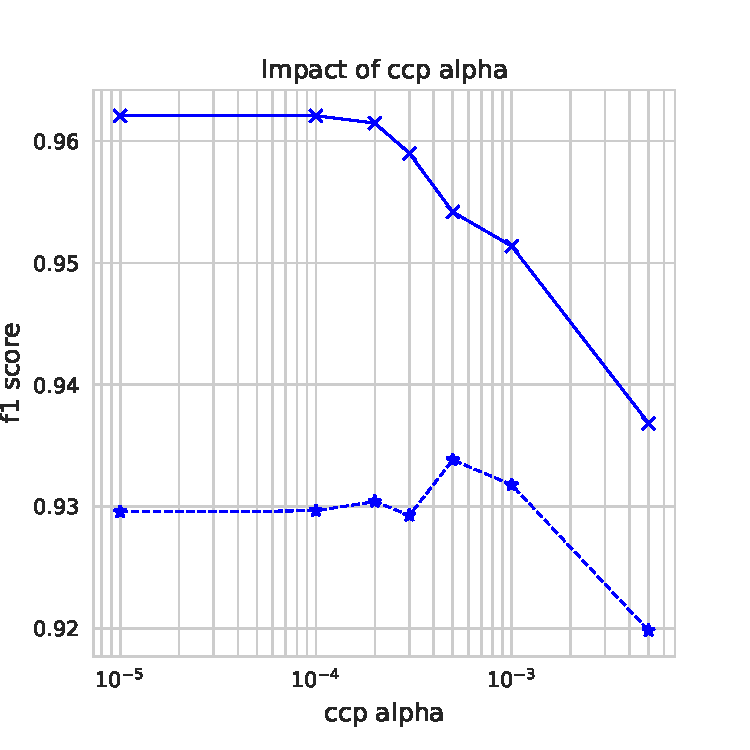
\includegraphics[width=1\linewidth]{email_spam/rnd_ccpalpha.pdf}
\end{minipage}
\begin{minipage}[l]{0.3\textwidth}
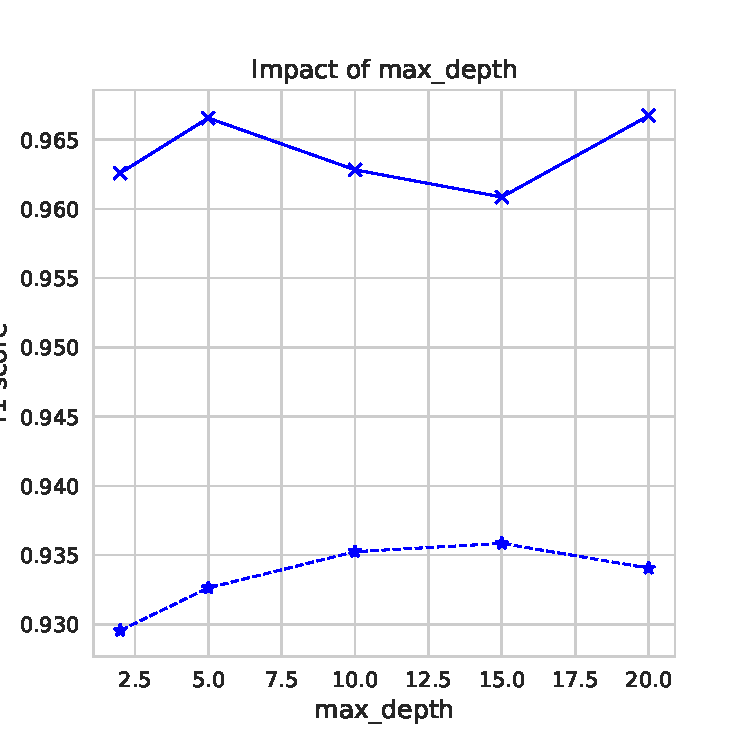
\includegraphics[width=1\linewidth]{email_spam/rnd_depth.pdf}
\end{minipage}
\begin{minipage}[l]{0.3\textwidth}
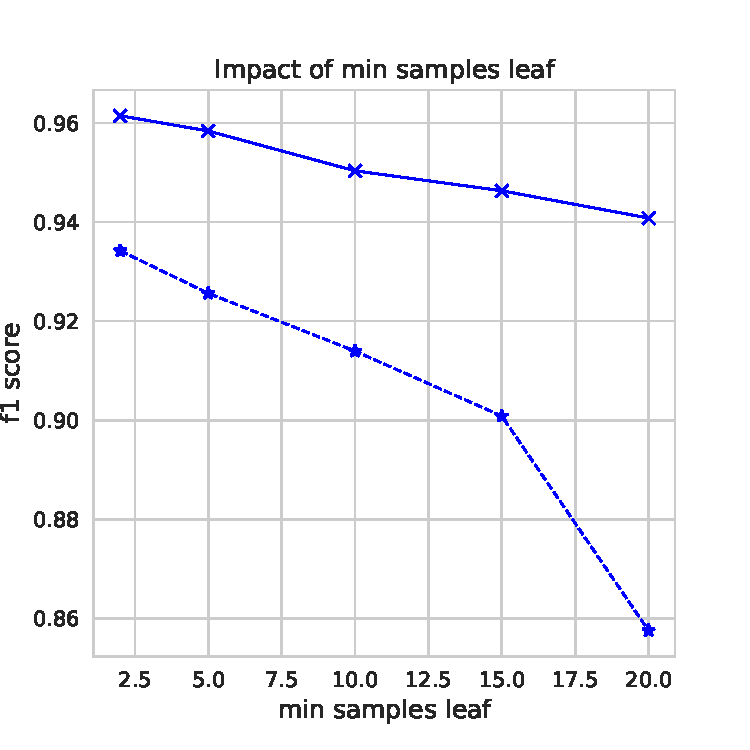
\includegraphics[width=1\linewidth]{email_spam/rnd_min_samples_leaf.pdf}
\end{minipage}
   \caption{F1-score of Random-Forrest for different pre-processing parameters and model-parameters}
\label{spamfig_fig2}
\end{figure}
%
The random forrest algorithm is usually not affected in its performance by scaling. Nevetheless we inspect the influence of the scaling parameters in \ref{spamfig_fig2} at top left with 8000 features extracted. We see that no scaling gives even for this algorithm less performance. Since the difference for the cross-validation is small we keep the unscaled data for this algorithm. When considering the impact of the number of extracted features in \ref{spamfig_fig2} top middle the f1-score in the cross validation improves till 7000 features are reached and then drops again. Therefore to decrease the runtime as much as we can we select 7000 features even if the holdout f1-score here is clearly lower. Another important parameter for performance and runtime in the random forrest is the number of trees that are build. The performance of this parameter can be seen in \ref{spamfig_fig2} top right. The performance increases when we build more decision trees but at 50 trees this preformance increase is not significant anymore. Therefore to decrease the runtime we select 50 trees for further investigations but 70 trees when stating the optimal parameters below. So far the decision trees are grown to full lenght and might overfit largly. In \ref{spamfig_fig2} bottom left we perform cost-complexity pruning on the tree. Larger values of the parameter will post-prune more tree branches. At $5e-3$ we reach an optimum in the cross validation f1-score which doesent differ significantly from the other performances achived for different values of this parameter. We still want to select parameter as large a possible to simplify the tree and prevent overfitting for the generqal case such that we select $5\cdot10^{-3}$ for this parameter. We can also prevent the tree from overfitting by bounding its depth. The impact of this method is shown in \label{spamfig_fig2} bottom right. Here we obtain a optimum for a maximal tree depth of $15$. The last parameter to prevent overfitting we investigate is the minimum number of spamples required to split a leaf into a new branch. This parameters performance impact can be seen in \ref{spamfig_fig2} bottom right. Here increasing the parameter values drastically decreases the f1-score and therefore we dont make use of it.

In our analysis we obtained the best performance with :scaling method: none, extracted features: $8000$, cost complexity pruning parameter $5\cdot10^{-3}$, maximum depth: $60$, number of trees: 70. By that we obtain on the testset a f1-score of $0.93$ for holdout and cross-validation with 5 validation steps.

\textbf{Naive Bayes}:
Since this algorithm has a much smaller runtime we again switch to evaluationg the peformance also on the testset and doing 10 validation steps in the cross-validation. In Naive Bayes the scaling the scaling is generally not an issue. If we nevetheless apply the different scaling methods (only the ones that produce positiv ranges) we observe the bahaviour shown in figure \ref{spamfig_fig3} left. Here 6000 features were extracted and the the logarithmic scaling is having the best performance wherein the minmax scaling is performing significantly worse than the other methods. We choose logarithmic scaling and proceed with evaluating the impact of the number of extracted features in figure \ref{spamfig_fig3}  middle. Here for the crossvalidation on the validation set the f1-score is monotonically increasing. Since the performance increase is not significant after usding more than 6000 features we use that number of features for this algorithm. The laplace smoothing parameters influence is plotted in figure \ref{spamfig_fig3} right. The impact of this parameter on the performance is not large but we can identify an optimum at a value of 1.

\begin{figure}
\begin{minipage}[l]{0.3\textwidth}
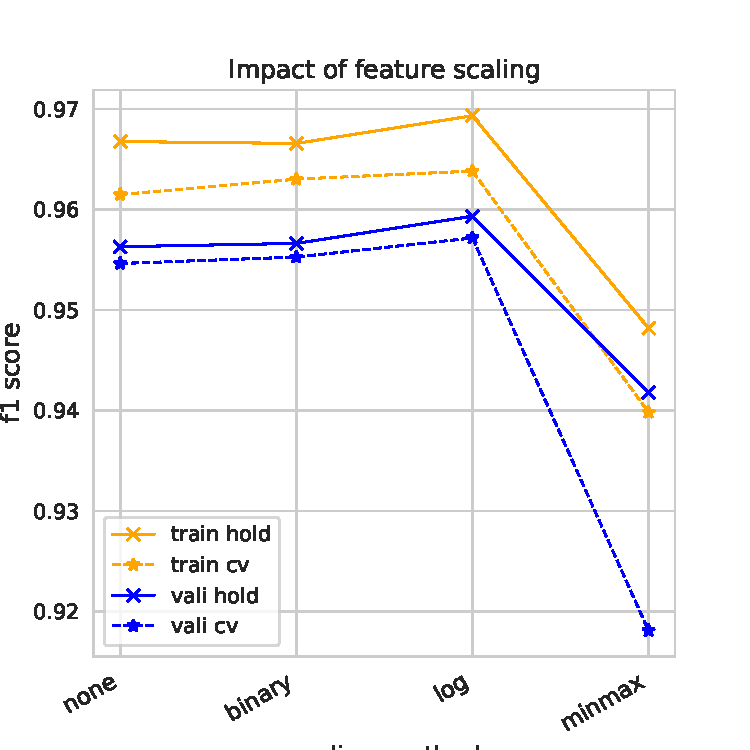
\includegraphics[width=1\linewidth]{email_spam/nb_scaling.pdf}
\end{minipage}
\begin{minipage}[l]{0.3\textwidth}
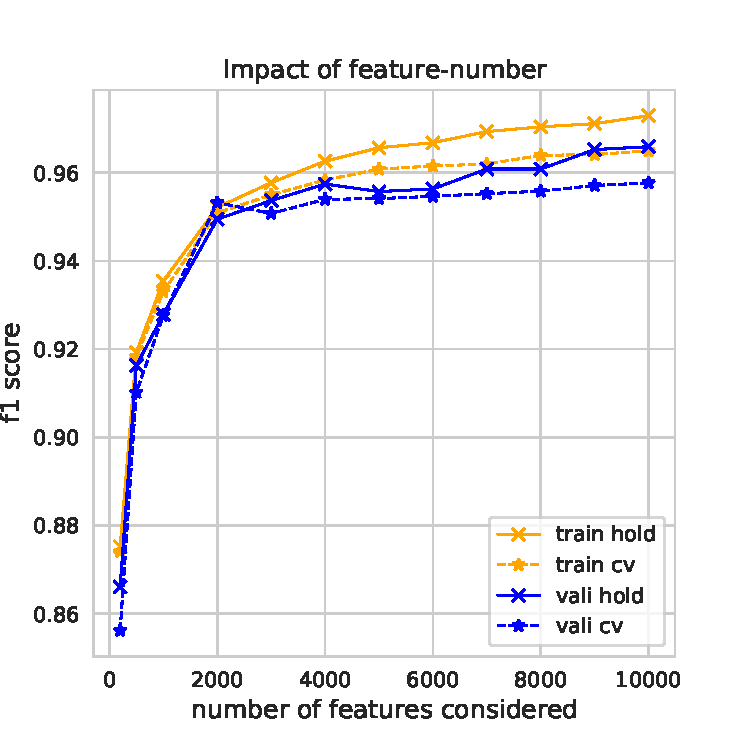
\includegraphics[width=1\linewidth]{email_spam/nb_features.pdf}
\end{minipage}
\begin{minipage}[l]{0.3\textwidth}
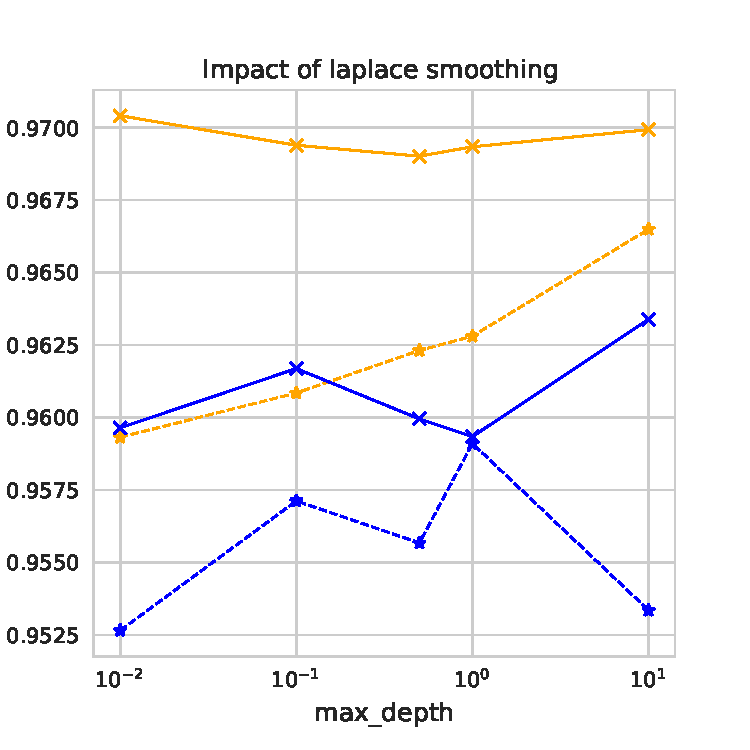
\includegraphics[width=1\linewidth]{email_spam/nb_smoother.pdf}
\end{minipage}
   \caption{F1-score of Naive Bayes for different pre-processing parameters and model-parameters}
\label{spamfig_fig3}
\end{figure}

The best parameters for the Naive Bayes algorithm are by that: :scaling method: logarithmic, extracted features: $6000$, smoothing parameter: $1$. This gives a $0.97$ f1-score on for the holdout validation and $0.96$ for the corssvalidation executed on the testset.


\subsection{Performance-Analysis}


\section{Bridges Dataset(\href{https://archive.ics.uci.edu/ml/datasets/Pittsburgh+Bridges}{link to dataset})}
\subsection{Dataset Description}
In this dataset with a size of 108 smaples, a collection of attributes of briges in Pittsburgh Pennsylvania is presented. The task is to predict the type of bridge by the given attributes. The the attributes are summarized in table \ref{bridgetab_tab0}, where we can see that most of them are nominal and lenght and span can be identified as ordinal. 
%
\begin{figure}
  \begin{tabular}{ | l | l | l | l |}
    \hline
    attribute & propertie 				    & attribute   & propertie 				\\ \hline
    1. river 		 & 3 nominal values 		    & 7. clear-g 		 & 2 nominal values			\\ \hline
    2. location 	 & 52 nominal values 		    & 8. t-or-d  	 & 2 nominal values			\\ \hline
    3. erected 		 & 4 nominal values 		    & 9. material  	 & 3 nominal values			\\ \hline
    4. purpose 		 & 4 nominal values 		    & 10. span  	& ordinal, short, medium, long			\\ \hline
    5. length 		 & ordinal, short, medium, long & 11. rel-l       & 3 nominal values			\\ \hline
    6. lanes		 & 4 nominal values	  			& 12. type		 & 6 nominal values 			\\ \hline
  \end{tabular}
  \caption{attributes for the bridges dataset}
  \label{bridgetab_tab0}
\end{figure}
%
In figure \ref{bridges_fig0} left we see the distribution of the type of bridges that occur in our data. 
This trainset is imbalanced, with a bit less than the half of the samples which are labellized as simple truss... we can already imagine that our results will not be very accurate according to the small amount of samples and this very imbalanced dataset (we only have around 10 samples per label in most of cases). 

\begin{figure}
\begin{minipage}[l]{0.3\textwidth}
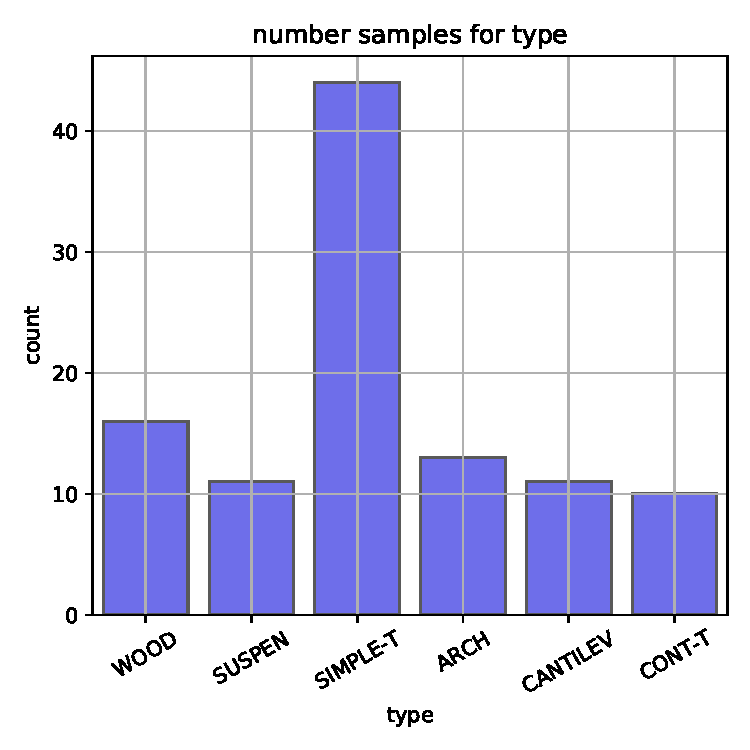
\includegraphics[width=1\linewidth]{bridges/classification_trainset.pdf}
\end{minipage}
\begin{minipage}[l]{0.3\textwidth}
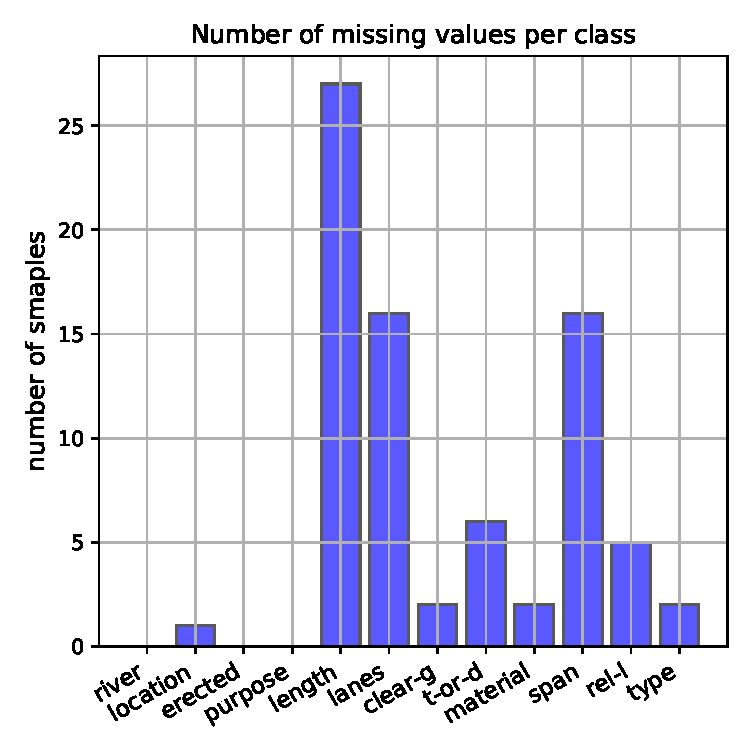
\includegraphics[width=1\linewidth]{bridges/bridges_missing.pdf}
\end{minipage}
\begin{minipage}[l]{0.3\textwidth}
\end{minipage}
   \caption{left: distribution of the target value over the dataset, middle: distribution of misssing values}
\label{bridges_fig0}
\end{figure}

Next in figure \ref{bridges_fig0} middle we show the missing values in the dataset. We can see that there are some missing values, and we have the repartition of missing values among samples with the following table {insert table}. We can notice that the feature "lenght" is the most incomplete one, with 25% missing values, and "lanes" and "span" have 15% missing values. The other features having less than 6% missing values. We can also notice that three labels are missing, so we have to drop it. We treat missing values by two approaches namely, replacing then with the value of the nearest neighbor smaple or randomly inserting another value for the missing one.
\subsection{Pre-Processing}
\subsection{Parameter-Tuning}
\subsection{Performance-Analysis}

\section{Conclusion}
%
\begin{figure}
\center
  \begin{tabular}{ | l | l | l | l | l |}
    \hline
    Dataset & Perceptron & Random Forrest  & Naive Bayes & validation method\\ \hline
    Amazon  & 0.43			   		 		 & 0.48\cellcolor{gray!25}   	 	   & 0.54\cellcolor{gray!50} & cross \\ \hline
	Email   & 0.95\cellcolor{gray!25}  	 	 & 0.93   		   					   & 0.96\cellcolor{gray!50} & cross \\ \hline
	Voting  & 0.93\cellcolor{gray!25}  	 	 & 0.97\cellcolor{gray!50}   		   & 0.88 	     		     & holdout \\ \hline
	Bridges & 0.53  	 				 	 & 0.60\cellcolor{gray!25}   		   & 0.66\cellcolor{gray!50} & holdout \\ \hline
  \end{tabular}
  \caption{Best f1-scores obtained on the testsets}
  \label{bridgetab_tab0}
\end{figure}
%
%Bibliography
\newpage
\bibliography{lib} 
\bibliographystyle{ieeetr}

\end{document}
